%%%%%%%%%%%%%%%%%%%%%%%%%%%%%%%%%%%%%%%%%
% Short Sectioned Assignment
% LaTeX Template
% Version 1.0 (5/5/12)
%
% This template has been downloaded from:
% http://www.LaTeXTemplates.com
%
% Original author:
% Frits Wenneker (http://www.howtotex.com)
%
% License:
% CC BY-NC-SA 3.0 (http://creativecommons.org/licenses/by-nc-sa/3.0/)
%
%%%%%%%%%%%%%%%%%%%%%%%%%%%%%%%%%%%%%%%%%

%----------------------------------------------------------------------------------------
%	PACKAGES AND OTHER DOCUMENT CONFIGURATIONS
%----------------------------------------------------------------------------------------

\documentclass[paper=a4, fontsize=11pt]{scrartcl} % A4 paper and 11pt font size

%\usepackage[T1]{fontenc} % Use 8-bit encoding that has 256 glyphs
%\usepackage[brazil]{babel}
%\usepackage[utf8]{inputenc}
%\usepackage[brazilian]{babel}
\usepackage{pgf,tikz}
\usepackage{pgfplots}
\usepackage[framemethod=TikZ]{mdframed}
\pgfplotsset{width=10cm, compat=newest}
\pgfplotsset{soldot/.style={color=blue,only marks,mark=*}} \pgfplotsset{holdot/.style={color=blue,fill=white,only marks,mark=*}}
\usetikzlibrary{arrows}
\usepackage[utf8]{inputenc} % Required for including letters with accents
\usepackage[T1]{fontenc} % Use 8-bit encoding that has 256 glyphs
\usepackage{subfigure}
\usepackage{wrapfig}
\usepackage{float}
\usepackage{multicol} % 
\usepackage{microtype} % Slightly tweak font spacing for aesthetics
\usepackage[margin=2cm]{geometry}
\usepackage{fourier} % Use the Adobe Utopia font for the document - comment this line to return to the LaTeX default
\usepackage[portuguese]{babel} % English language/hyphenation
\usepackage{amsmath,amsfonts,amsthm} % Math packages
\usepackage{hyperref}
\usepackage{cancel}
\usepackage[breakable]{tcolorbox}
\tcbset{lowerbox=invisible,savelowerto=\jobname_bspsave.tex,colback=white}

\usepackage{amsmath}
\usepackage{sectsty} % Allows customizing section commands
\allsectionsfont{\centering \normalfont\scshape\bfseries} % Make all sections centered, the default font and small caps

\subsectionfont{\normalfont\scshape\bfseries}
\subsubsectionfont{\normalfont\scshape\bfseries}
\usepackage{fancyhdr} % Custom headers and footers
\pagestyle{fancyplain} % Makes all pages in the document conform to the custom headers and footers
\fancyhead{} % No page header - if you want one, create it in the same way as the footers below
\fancyfoot[L]{} % Empty left footer
\fancyfoot[C]{} % Empty center footer
\fancyfoot[R]{\thepage} % Page numbering for right footer
\renewcommand{\headrulewidth}{0pt} % Remove header underlines
\renewcommand{\footrulewidth}{0pt} % Remove footer underlines
\setlength{\headheight}{13.6pt} % Customize the height of the header

\numberwithin{equation}{section} % Number equations within sections (i.e. 1.1, 1.2, 2.1, 2.2 instead of 1, 2, 3, 4)
\numberwithin{figure}{section} % Number figures within sections (i.e. 1.1, 1.2, 2.1, 2.2 instead of 1, 2, 3, 4)
\numberwithin{table}{section} % Number tables within sections (i.e. 1.1, 1.2, 2.1, 2.2 instead of 1, 2, 3, 4)

\setlength\parindent{0pt} % Removes all indentation from paragraphs - comment this line for an assignment with lots of text


% new
\mdfsetup{skipabove=\topskip,skipbelow=\topskip}
%%% upto here
\newcounter{theo}[section]
\newenvironment{theo}[1][]{%
\stepcounter{theo}%
\ifstrempty{#1}%
 {\mdfsetup{%
   frametitle={%
    \tikz[baseline=(current bounding box.east),outer sep=0pt]
    \node[anchor=east,rectangle,fill=blue!20]
         {\strut Resumo~\thetheo};}}
 }%
{\mdfsetup{%
  frametitle={%
   \tikz[baseline=(current bounding box.east),outer sep=0pt]
   \node[anchor=east,rectangle,fill=blue!20]
        {\strut Resumo~\thetheo};}}%
 }%
\mdfsetup{innertopmargin=10pt,linecolor=blue!20,%
       linewidth=2pt,topline=true,
       frametitleaboveskip=\dimexpr-\ht\strutbox\relax,}
   \begin{mdframed}[]\relax%
}
{\end{mdframed}}

% theorem

\newtheorem{teorema}{Teorema}
\newtheorem{prop}{Proposição}
\newtheorem{defi}{Definição}

% inserir figura dentro de colunas
\newenvironment{Figure}
  {\par\medskip\noindent\minipage{\linewidth}}
  {\endminipage\par\medskip}
  
  
% linha entrre colunas
% \setlength{\columnseprule}{1pt}
% \def\columnseprulecolor{\color{black}}
%----------------------------------------------------------------------------------------
%	TITLE SECTION
%----------------------------------------------------------------------------------------
\usepackage{authblk}
\usepackage{blindtext}

\begin{document}
\newcommand{\horrule}[1]{\rule{\linewidth}{#1}} % Create horizontal rule command with 1 argument of height

\title{	
\normalfont \normalsize 
\textsc{UFRPE - Departamaento de Matemática} \\ [25pt] % Your university, school and/or department name(s)
\horrule{0.5pt} \\[0.1cm] % Thin top horizontal rule
\huge Lista de Exercícios Cálculo NI: Parte II \\ % The assignment title
\horrule{2pt} \\[0.5cm] % Thick bottom horizontal rule
}

\author{Leon Silva\\\href{mailto:leon.silva@ufrpe.br}{\textcolor{blue}{leon.silva@ufrpe.br}}} % Your name

\date{\normalsize\today} % Today's date or a custom date



\maketitle % Print the title

%----------------------------------------------------------------------------------------
%	PROBLEM 1
%----------------------------------------------------------------------------------------
%% Parte I
\section{Números reais}

\begin{multicols}{2}
\subsubsection*{Propriedades}

Dados $x,y,z,w \in \mathbb{R}$:\\
$x<y \iff x+z < y+z$\\
$z>0 \iff z^{-1}>0$\\
$z>0 \iff -z<0$\\
se  $z>0, x<y \iff xz<yz$\\
$z<0, x<y \iff xz>yz$

\subsubsection*{\textcolor{red}{Atenção!}}

Dados $x,y,z,w \in \mathbb{R}$:
\begin{multicols}{2}
$\dfrac{xy + z}{x}\neq y+z$\\[0.15cm]
$\dfrac{x}{y+z}\neq \dfrac{x}{y}+\dfrac{x}{z}$\\[0.15cm]
$\dfrac{x+y}{z+w}\neq \dfrac{x}{y}+\dfrac{z}{w}$\\[0.15cm]
$\sqrt{a+b}\neq \sqrt{a}+\sqrt{b}$\\[0.15cm]
$\sqrt{a^2+b^2}\neq a+b$\\
\end{multicols}
\end{multicols}

\section{Funções}
%\subsection{Funções, Domínio e Imagem}
\subsection*{Conceitos Básicos}
\begin{tcolorbox}

\begin{defi} Uma função de variável real a valores reais é uma função $f:X\longrightarrow \mathbb{R}$, onde $X\subset \mathbb{R}$. O conjunto $X$ é o domínio de $f$ e indica-se por $D_f$, ou seja, $D_f=X$. O conjunto dos números reais é o contradomínio. A imagem é o subconjunto  de $\mathbb{R}$, indicado por $\textrm{Im}_f$ e definido por $f(X)=\textrm{Im}_f=\{y\in\mathbb{R}: y=f(x), x\in X\}$.
\end{defi}

\begin{defi}Seja $f:X\longrightarrow \mathbb{R}$ uma função. O conjunto $G_f=\left\{(x,f(x))\in\mathbb{R}^2: x\in X\right\}$ denomina-se \textbf{gráfico} de $f$.
\end{defi}



\begin{defi}

Uma função $f: X \rightarrow \mathbb{R}$  é dita \textbf{injetora} (injetiva)  se para cada $y\in\mathrm{Im}_f,$ existe um único $x\in D_f=X$ tal que $f(x)=y.$
Ou seja, se $$f(x_1)=f(x_2)\Rightarrow x_1=x_2, \forall x_1, x_2\in\mathrm{D}_f.$$
\end{defi}
% \begin{defi}Função composta
% \begin{figure}
%     \centering
%     \begin{tikzpicture}[ scale=0.5]
\clip(-4.3,-3.2) rectangle (10.14,6.3);
\draw (-3,2)-- (-1,2);
\draw (0,2)-- (2,2);
\draw (3,2)-- (5,2);
\draw [shift={(-0.46,1.6)}] plot[domain=0.73:2.53,variable=\t]({1*1.23*cos(\t r)+0*1.23*sin(\t r)},{0*1.23*cos(\t r)+1*1.23*sin(\t r)});
\draw [shift={(2.48,1.66)}] plot[domain=0.56:2.5,variable=\t]({1*1.2*cos(\t r)+0*1.2*sin(\t r)},{0*1.2*cos(\t r)+1*1.2*sin(\t r)});
\draw [shift={(0.94,3.84)}] plot[domain=3.79:5.66,variable=\t]({1*3.72*cos(\t r)+0*3.72*sin(\t r)},{0*3.72*cos(\t r)+1*3.72*sin(\t r)});
\draw (-2.92,1.9) node[anchor=north west] {A};
\draw (0.1,1.86) node[anchor=north west] {B};
\draw (3.08,1.84) node[anchor=north west] {C};
\draw (2.54,3.34) node[anchor=north west] {f};
\draw (-0.58,3.28) node[anchor=north west] {g};
\draw (0.7,0.32) node[anchor=north west] {$f\circ g$};
\begin{scriptsize}
\fill [color=black] (-3,2) circle (0.5pt);
\fill [color=black] (-1,2) circle (0.5pt);
\fill [color=black] (0,2) circle (0.5pt);
\fill [color=black] (2,2) circle (0.5pt);
\fill [color=black] (3,2) circle (0.5pt);
\fill [color=black] (5,2) circle (0.5pt);
\fill [color=black,shift={(0.46,2.42)},rotate=180] (0,0) ++(0 pt,2.25pt) -- ++(1.95pt,-3.375pt)--++(-3.9pt,0 pt) -- ++(1.95pt,3.375pt);
\fill [color=black,shift={(3.5,2.3)},rotate=180] (0,0) ++(0 pt,2.25pt) -- ++(1.95pt,-3.375pt)--++(-3.9pt,0 pt) -- ++(1.95pt,3.375pt);
\fill [color=black,shift={(3.96,1.68)}] (0,0) ++(0 pt,2.25pt) -- ++(1.95pt,-3.375pt)--++(-3.9pt,0 pt) -- ++(1.95pt,3.375pt);
\end{scriptsize}
\end{tikzpicture}
% \end{figure}
%\end{defi}
\begin{defi}
Seja $f: X \longrightarrow \mathbb{R}$ uma injetora. Então, a sua inversa $f^{-1}: f(X) \longrightarrow X$ é definida por  
\begin{align*}
    f^{-1}(y) \iff f(x)=y \quad  \forall y\in f(X)
\end{align*}
\end{defi}

\begin{defi}
Uma função $f: X \rightarrow \mathbb{R}$ é dita \textbf{sobrejetora} (sobrejetiva) se $f(X)=\mathbb{R}$.
\end{defi}
\begin{defi}
Uma função $f: X \rightarrow \mathbb{R}$ é dita \textbf{bijetora} (bijetiva) se é injetora e sobrejetora.
\end{defi}



\begin{defi}
Uma função $f: X \longrightarrow\mathbb{R}, X\subset\mathbb{R},$ é
dita \textbf{monótona} se ela preserva (ou inverte) a relação de
ordem. Sejam $x_1,x_2\in \mathbb{R}$, dizemos que $f$ é monótona
\begin{enumerate}
\item [(i)] \textbf{crescente} ou \textbf{estritamente crescente}, quando
$x_1<x_2 \Rightarrow f(x_1)<f(x_2)$
\item [(ii)]\textbf{decrescente} ou \textbf{estritamente decrescente}, quando
$x_1<x_2 \Rightarrow f(x_1)>f(x_2)$
\item [(iii)] \textbf{não-decrescente}, quando
$x_1<x_2 \Rightarrow f(x_1)\leq f(x_2)$
\item [(iv)]\textbf{monótona não-crescente}, quando
$x_1<x_2 \Rightarrow f(x_1)\geq f(x_2)$
\end{enumerate}
\end{defi}
\end{tcolorbox}

\begin{tcolorbox}

\subsubsection*{Paridade de Funções}
\begin{defi} Se $D_{f} \subseteq \mathbb{R}$ simétrico em relação à origem. Então $f$ é dita \textbf{par} se  $f(-x) = f(x), \forall x \in D_f$ e \textbf{impar} se $f(-x) = -f(x), \forall x \in D_f$.

\begin{figure}[H]
\centering
\subfigure{
    \begin{tikzpicture}[scale=0.5]
\begin{axis}[
 axis lines=middle,
 ticklabel style={fill=white},
%  xmin=-4,xmax=4,
 ymin=-1,ymax=1,
 xlabel=$x$,ylabel=$y$,
 domain=-4:4,
 samples=100,
 smooth,
 xtick={-1.5,0,1.5}, ytick={-1,1},
 xticklabels={$-a$,0,$a$}, yticklabels={,,},
 width=10cm]
\coordinate  (x2) at (1,1);
\coordinate  (x1) at (-1,-1);
\addplot[blue] {0.5*sin(deg(x))};

\draw[dashed] (-1.5,0) --(-1.5,{0.5*sin(deg(-1.5)}) --(0,{0.5*sin(deg(-1.5)}) ;

\draw[dashed] (1.5,0)  -- (1.5,{0.5*sin(deg(1.5)})--(0, {0.5*sin(deg(1.5)});
\node[] at (axis cs:2.2,0.7) {função impar};

\node[right] at (axis cs:0, {0.5*sin(deg(-1.5))}) {$-f(a)$};
\node[left] at (axis cs:0, {0.5*sin(deg(1.5))}) {$f(a)$};
\end{axis}
\end{tikzpicture}}
    \qquad
\subfigure{
\begin{tikzpicture}[scale=0.5]
\begin{axis}[
 axis lines=middle,
 ticklabel style={fill=white},
%  xmin=-4,xmax=4,
 ymin=-0.5,ymax=2,
 xlabel=$x$,ylabel=$y$,
 domain=-4:4,
 samples=100,
 smooth,
 xtick={-1.5,0,1.5}, ytick={1},
 yticklabels={,,},   xticklabels={$-a$,0,$a$},
 width=10cm]
\coordinate  (x2) at (1,1);
\coordinate  (x1) at (-1,-1);
\addplot[blue] {1+0.5*cos(deg(x))};

\draw[dashed] (-1.5,0) --(-1.5,{1+0.5*cos(deg(-1.5)}) -- (1.5,{1+0.5*cos(deg(1.5)})--(1.5,0) ;
\node[] at (axis cs:2.2,1.5) {função par};
\end{axis}
\end{tikzpicture}}
\end{figure}
\end{defi}
\end{tcolorbox}
\begin{tcolorbox}


\subsubsection*{Funções potência $f(x)=x^p$}

% \begin{enumerate}
%     \item $f(x)=x^n$, $n \in \mathrm{Z}_{+}$
%     \begin{figure}[H]
% \centering
%     \subfigure[][$n$ par]{
%     \begin{tikzpicture}[scale=0.5]
\begin{axis}[
  %title = {$f(x)=x^n$, $n=2k$, $k \in \mathrm{Z}_{+}$},
 axis lines=middle,
 ticklabel style={fill=white},
 xmin=-2.5,xmax=2.6,
 ymin=-0.5,ymax=6,
 xlabel=$x$,ylabel=$y$,
 domain=-2:2,
 samples=100,
 smooth,
 xtick={-1,0,1},ytick={1},
 yticklabels={,,},   xticklabels={,,},
 width=10cm, height=8cm]
\coordinate  (x2) at (1,1);
\coordinate (x1) at (-1,1);

\addplot[black] { x^2};
\addplot[gray] {x^4};
\addplot[blue] {x^6};
\fill[black] (x1) circle (1.5pt);
\fill[black] (x2) circle (1.5pt);

\node[pin= 20:{$y=x^2$}] at (axis cs:1.2,{(1.2)^2}) {};
\node[pin= 50:{$y=x^4$}] at (axis cs:1.4,{(1.4)^4}) {};
\node[pin= 160:{$y=x^6$}] at (axis cs:1.2,{(1.2)^6}) {};
\node[right] at (x2) {$(1,1)$};
\node[left] at (x1) {$(-1,1)$};
\end{axis}
\end{tikzpicture}














}
%     \qquad\qquad
%     \subfigure[][$n$ impar]{
%     \begin{tikzpicture}[scale=0.5]
\begin{axis}[
%title = {$f(x)=x^n$, $n=2k+1$, $k \in \mathrm{Z}_{+}$},
 axis lines=middle,
 ticklabel style={fill=white},
 xmin=-2.5,xmax=2.6,
 ymin=-6,ymax=6,
 xlabel=$x$,ylabel=$y$,
 domain=-2:2,
 samples=100,
 smooth,
 xtick={-1,0,1},ytick={1},
 yticklabels={,,},   xticklabels={,,},
 width=10cm, height=8cm]
\coordinate  (x2) at (1,1);
\coordinate (x1) at (-1,-1);

\addplot[black] { x^3};
\addplot[blue] {x^5};

\fill[black] (x1) circle (1.5pt);
\fill[black] (x2) circle (1.5pt);

\node[pin= 20:{$y=x^3$}] at (axis cs:1.2,{(1.2)^3}) {};
\node[pin= 180:{$y=x^5$}] at (axis cs:1.4,{(1.4)^5}) {};

\node[right] at (x2) {$(1,1)$};
\node[left] at (x1) {$(-1,-1)$};
\end{axis}
\end{tikzpicture}}
% \end{figure}

% \item $f(x)=x^{1/n}=\sqrt[n]{x}$, $n \in \mathrm{Z}_{+}$
% \begin{figure}[H]
% \centering
%     \subfigure{
%     \begin{tikzpicture}[scale=0.5]
\begin{axis}[
 %title={$f(x)=x^{1/n}=\sqrt[n]{x}$, $n \in \mathrm{Z}_{+}$}
 axis lines=middle,
 ticklabel style={fill=white},
 xmin=-1,xmax=1.5,
 ymin=-0.5,ymax=1.5,
 xlabel=$x$,ylabel=$y$,
 domain=0:1.5,
 samples=100,
 smooth,
 xtick={-1,0,1},ytick={1},
 yticklabels={,,},   xticklabels={,,},
 width=10cm, height=6cm]
\coordinate  (x2) at (1,1);

\addplot[blue] { sqrt(x)};

\fill[black] (x2) circle (1.5pt);

\node[] at (axis cs:0.9,{(0.9)^(1/2)+0.4}) {$y=\sqrt{x}$};

\node[below right] at (x2) {$(1,1)$};

\end{axis}
\end{tikzpicture}
}
%     \qquad\qquad
%     \subfigure{
%     \begin{tikzpicture}[scale=0.5]
\begin{axis}[
 axis lines=middle,
 ticklabel style={fill=white},
 xmin=-1.5,xmax=1.5,
 ymin=-1.5,ymax=1.5,
 xlabel=$x$,ylabel=$y$,
 domain=-1.5:1.5,
 samples=100,
 smooth,
 xtick={-1,0,1},ytick={1},
 yticklabels={,,},   xticklabels={,,},
 width=10cm, height=6cm]
\coordinate  (x2) at (1,1);

\addplot[blue] {x/abs(x)*abs(x)^(1/3)};

\fill[black] (x2) circle (1.5pt);

\node[] at (axis cs:0.9,{(0.9)^(1/3)+0.4}) {$y=\sqrt[3]{x}$};
\node[below right] at (x2) {$(1,1)$};

\end{axis}
\end{tikzpicture}}
% \end{figure}

% \item $f(x)=x^{n}$, $n \in \mathrm{Z}_{-}$
% \begin{figure}[H]
%     \centering
%     \subfigure{
%     \begin{tikzpicture}[scale=0.5]
\begin{axis}[
 axis lines=middle,
 ticklabel style={fill=white},
 xmin=-1.5,xmax=1.5,
 ymin=-4,ymax=4,
 xlabel=$x$,ylabel=$y$,
 domain=-1.5:1.5,
 samples=100,
 smooth,
 xtick={-1,0,1},ytick={1,-1},
 yticklabels={,,},   xticklabels={,,},
 width=10cm]
\coordinate  (x2) at (1,1);
\coordinate  (x1) at (-1,-1);
\addplot[blue] {1/x};


\fill[black] (x2) circle (1.5pt);
\fill[black] (x1) circle (1.5pt);

\node[] at (axis cs:0.8,{1/(0.8)+1}) {$y=\dfrac{1}{x}$};

\node[above right] at (x2) {$(1,1)$};
\node[above right] at (x1) {$(-1,-1)$};

\end{axis}
\end{tikzpicture}}
%     \qquad\qquad
%     \subfigure{
% \begin{tikzpicture}[scale=0.5]
\begin{axis}[
 axis lines=middle,
 ticklabel style={fill=white},
 xmin=-1.5,xmax=1.5,
 ymin=-1,ymax=5,
 xlabel=$x$,ylabel=$y$,
 domain=-1.4:1.4,
 samples=30,
 smooth,
 xtick={-1,0,1},ytick={1},
 yticklabels={,,},   xticklabels={,,},
 width=10cm]
\coordinate  (x2) at (1,1);
\coordinate  (x1) at (-1,1);
\addplot[blue] {1/x^2};


\fill[black] (x2) circle (1.5pt);
\fill[black] (x1) circle (1.5pt);

\node[] at (axis cs:0.9,{1/(0.8)^2+1.5}) {$y=\dfrac{1}{x^2}$};


\node[above right] at (x2) {$(1,1)$};
\node[above left] at (x1) {$(-1,1)$};
\end{axis}
\end{tikzpicture}}
% \end{figure}

% \end{enumerate}

\begin{figure}[H]
\centering
    \subfigure{
    \begin{tikzpicture}[scale=0.5]
\begin{axis}[
  %title = {$f(x)=x^n$, $n=2k$, $k \in \mathrm{Z}_{+}$},
 axis lines=middle,
 ticklabel style={fill=white},
 xmin=-2.5,xmax=2.6,
 ymin=-0.5,ymax=6,
 xlabel=$x$,ylabel=$y$,
 domain=-2:2,
 samples=100,
 smooth,
 xtick={-1,0,1},ytick={1},
 yticklabels={,,},   xticklabels={,,},
 width=10cm, height=8cm]
\coordinate  (x2) at (1,1);
\coordinate (x1) at (-1,1);

\addplot[black] { x^2};
\addplot[gray] {x^4};
\addplot[blue] {x^6};
\fill[black] (x1) circle (1.5pt);
\fill[black] (x2) circle (1.5pt);

\node[pin= 20:{$y=x^2$}] at (axis cs:1.2,{(1.2)^2}) {};
\node[pin= 50:{$y=x^4$}] at (axis cs:1.4,{(1.4)^4}) {};
\node[pin= 160:{$y=x^6$}] at (axis cs:1.2,{(1.2)^6}) {};
\node[right] at (x2) {$(1,1)$};
\node[left] at (x1) {$(-1,1)$};
\end{axis}
\end{tikzpicture}














}
    \qquad
    \subfigure{
    \begin{tikzpicture}[scale=0.5]
\begin{axis}[
%title = {$f(x)=x^n$, $n=2k+1$, $k \in \mathrm{Z}_{+}$},
 axis lines=middle,
 ticklabel style={fill=white},
 xmin=-2.5,xmax=2.6,
 ymin=-6,ymax=6,
 xlabel=$x$,ylabel=$y$,
 domain=-2:2,
 samples=100,
 smooth,
 xtick={-1,0,1},ytick={1},
 yticklabels={,,},   xticklabels={,,},
 width=10cm, height=8cm]
\coordinate  (x2) at (1,1);
\coordinate (x1) at (-1,-1);

\addplot[black] { x^3};
\addplot[blue] {x^5};

\fill[black] (x1) circle (1.5pt);
\fill[black] (x2) circle (1.5pt);

\node[pin= 20:{$y=x^3$}] at (axis cs:1.2,{(1.2)^3}) {};
\node[pin= 180:{$y=x^5$}] at (axis cs:1.4,{(1.4)^5}) {};

\node[right] at (x2) {$(1,1)$};
\node[left] at (x1) {$(-1,-1)$};
\end{axis}
\end{tikzpicture}}
    \subfigure{
    \begin{tikzpicture}[scale=0.5]
\begin{axis}[
 %title={$f(x)=x^{1/n}=\sqrt[n]{x}$, $n \in \mathrm{Z}_{+}$}
 axis lines=middle,
 ticklabel style={fill=white},
 xmin=-1,xmax=1.5,
 ymin=-0.5,ymax=1.5,
 xlabel=$x$,ylabel=$y$,
 domain=0:1.5,
 samples=100,
 smooth,
 xtick={-1,0,1},ytick={1},
 yticklabels={,,},   xticklabels={,,},
 width=10cm, height=6cm]
\coordinate  (x2) at (1,1);

\addplot[blue] { sqrt(x)};

\fill[black] (x2) circle (1.5pt);

\node[] at (axis cs:0.9,{(0.9)^(1/2)+0.4}) {$y=\sqrt{x}$};

\node[below right] at (x2) {$(1,1)$};

\end{axis}
\end{tikzpicture}
}
    \qquad
    \subfigure{
    \begin{tikzpicture}[scale=0.5]
\begin{axis}[
 axis lines=middle,
 ticklabel style={fill=white},
 xmin=-1.5,xmax=1.5,
 ymin=-1.5,ymax=1.5,
 xlabel=$x$,ylabel=$y$,
 domain=-1.5:1.5,
 samples=100,
 smooth,
 xtick={-1,0,1},ytick={1},
 yticklabels={,,},   xticklabels={,,},
 width=10cm, height=6cm]
\coordinate  (x2) at (1,1);

\addplot[blue] {x/abs(x)*abs(x)^(1/3)};

\fill[black] (x2) circle (1.5pt);

\node[] at (axis cs:0.9,{(0.9)^(1/3)+0.4}) {$y=\sqrt[3]{x}$};
\node[below right] at (x2) {$(1,1)$};

\end{axis}
\end{tikzpicture}}
    \subfigure{
    \begin{tikzpicture}[scale=0.5]
\begin{axis}[
 axis lines=middle,
 ticklabel style={fill=white},
 xmin=-1.5,xmax=1.5,
 ymin=-4,ymax=4,
 xlabel=$x$,ylabel=$y$,
 domain=-1.5:1.5,
 samples=100,
 smooth,
 xtick={-1,0,1},ytick={1,-1},
 yticklabels={,,},   xticklabels={,,},
 width=10cm]
\coordinate  (x2) at (1,1);
\coordinate  (x1) at (-1,-1);
\addplot[blue] {1/x};


\fill[black] (x2) circle (1.5pt);
\fill[black] (x1) circle (1.5pt);

\node[] at (axis cs:0.8,{1/(0.8)+1}) {$y=\dfrac{1}{x}$};

\node[above right] at (x2) {$(1,1)$};
\node[above right] at (x1) {$(-1,-1)$};

\end{axis}
\end{tikzpicture}}
    \qquad\qquad
    \subfigure{
\begin{tikzpicture}[scale=0.5]
\begin{axis}[
 axis lines=middle,
 ticklabel style={fill=white},
 xmin=-1.5,xmax=1.5,
 ymin=-1,ymax=5,
 xlabel=$x$,ylabel=$y$,
 domain=-1.4:1.4,
 samples=30,
 smooth,
 xtick={-1,0,1},ytick={1},
 yticklabels={,,},   xticklabels={,,},
 width=10cm]
\coordinate  (x2) at (1,1);
\coordinate  (x1) at (-1,1);
\addplot[blue] {1/x^2};


\fill[black] (x2) circle (1.5pt);
\fill[black] (x1) circle (1.5pt);

\node[] at (axis cs:0.9,{1/(0.8)^2+1.5}) {$y=\dfrac{1}{x^2}$};


\node[above right] at (x2) {$(1,1)$};
\node[above left] at (x1) {$(-1,1)$};
\end{axis}
\end{tikzpicture}}
\end{figure}
\end{tcolorbox}
% \subsubsection*{Função Módulo}
% Seja $x,y \in \mathbb{R}$ então:
% \begin{align*}
%     |x|=\begin{cases}
%      x \quad \text{se} \quad x\leq 0  \\
%      -x\quad \text{se} \quad x< 0
%     \end{cases}
% \end{align*}

% \begin{multicols}{2}
% \subsubsection*{Propriedades}
% $|xy|=|x||y|$\\
% $\left|\dfrac{x}{y}\right|=\dfrac{|x|}{|y|}$\\
% $|x^n|=|x|^n$\\
% $\sqrt{x^2}=|x|$\\
% $|x+y|\leq |x|+|y|$ \qquad (desigualdade triangular)
% \columnbreak
% \subsubsection*{Gráfico}
% \begin{Figure}
%     \begin{tikzpicture}[scale=0.5]
\begin{axis}[
 axis lines=middle,
 ticklabel style={fill=white},
 xmin=-1.5,xmax=1.5,
 ymin=-0.5,ymax=1.5,
 xlabel=$x$,ylabel=$y$,
 domain=-1.2:1.2,
 samples=100,
 smooth,
 xtick={-1,0,1},ytick={1},
 yticklabels={,,},   xticklabels={,,},
 width=10cm]
\coordinate  (x2) at (1,1);
\coordinate  (x1) at (-1,-1);
\addplot[blue] {abs(x)};

\node[] at (axis cs:0.8,1.2) {$y=|x|$};
\end{axis}
\end{tikzpicture}
% \end{Figure}
% \end{multicols}



\subsection*{Logaritmo e Exponencial}
\begin{tcolorbox}
Se $x, y >0$,$a>0$ e $\neq 0$, então:
\begin{align*}
    &\log_ax =y  \iff a^y=x\\
    &\ln{x}=\log_e{x}, \quad \text{onde} \quad \ln{e}=1\\
    &\ln{x}=y \iff  e^y=x
\end{align*}
%$$$$
\begin{multicols}{2}
\subsubsection*{Propriedades: Logaritmo}
 $\log_{a}(xy)=\log_{a}x + \log_{a}y$\\[0.1cm]
 $\log_{a}(\frac{x}{y})=\log_{a}x  \log_{a}y$\\[0.1cm]
 $\log_{a}(x^y)=y\log_{a}x$\\[0.1cm]
$\log_{a}c=\frac{\log_{b}c}{\log_{b}a}$\\[0.1cm]
 $a^{\log_a x}=a$\\[0.1cm]
 $\log_aa^x =x$%\\[0.2cm]

 \subsubsection*{Gráficos}
 \begin{Figure}
     \begin{tikzpicture}[scale=0.5]
\begin{axis}[
 axis lines=middle,
 ticklabel style={fill=white},
xmin=-1.,%xmax=1.5,
%ymin=-1,ymax=5,
 xlabel=$x$,ylabel=$y$,
 domain=0:5,
 samples=30,
 smooth,
 xtick={1},ytick={1},
 yticklabels={1},   xticklabels={1},
 width=10cm]
\coordinate  (x2) at (1,e);
\coordinate  (x1) at (1,0);
\addplot[blue] {ln(x)};
\addplot[red] {(ln(x)/ln(0.5))};
\fill[black] (x2) circle (1.5pt);
\fill[black] (x1) circle (1.5pt);

\node[] at (axis cs:1,{1.5}) {$y=\log_a{x}$};

\node[pin= 50:{$a>0$}] at (axis cs:3,{ln(3)}) {};
\node[pin= 50:{$0<a<1$}] at (axis cs:3,{(ln(3)/ln(0.5)}) {};
\end{axis}
\end{tikzpicture}
 \end{Figure}
\end{multicols}
 \end{tcolorbox}
\begin{tcolorbox}

\begin{multicols}{2}
\subsubsection*{Propriedades: Exponencial}
 $a^{-x}=\dfrac{1}{a^x}$\\
 $(a^x)^y=a^{xy}$\\
 $a^xa^y=a^{x+y}$\\
 $(ab)^x=a^xb^x, \forall b>0$\\
 $a^0=1$\\
 se $a>1,x<y \implies a^x < a^y$ \\
 se $0<x<1\implies a^x> a^y$
 \subsubsection*{Gráficos}
 \begin{Figure}
     \begin{tikzpicture}[scale=0.5]
\begin{axis}[
 axis lines=middle,
 ticklabel style={fill=white},
xmin=-5.,%xmax=1.5,
ymin=-1,ymax=5,
 xlabel=$x$,ylabel=$y$,
 domain=-5:5,
 samples=30,
 smooth,
 xtick={2.7182},ytick={1},
 yticklabels={1},   xticklabels={,,},
 width=10cm]
\coordinate  (x2) at (e,1);
\coordinate  (x1) at (0,1);
\addplot[blue] {2^(x)};
\addplot[red] {(1/2)^x)};
% \fill[black] (x2) circle (1.5pt);
% \fill[black] (x1) circle (1.5pt);

%\draw[dashed] (x1)--(x2) --(e,0);
\node[] at (axis cs:2.5,{3}) {$y=a^{x}$};

\node[pin= 50:{$a>0$}] at (axis cs:2,{2^(2)}) {};
\node[pin= 130:{$0<a<1$}] at (axis cs:-2,{(1/2)^(-2)}) {};
\end{axis}
\end{tikzpicture}
 \end{Figure}
\end{multicols}
\end{tcolorbox}

\subsection*{Trigonometria}
\begin{tcolorbox}
\begin{multicols}{2}
\subsubsection*{Identidades fundamentais}
$\cos^2{x}+\sin^2{x}=1$\\[0.15cm]
$1+\tan^2{x} = \sec^2{x} $\\[0.15cm]
$\sin(-x)=-\sin(x)$\\[0.15cm]
$\cos(-x)=\cos(x)$ \\[0.15cm]
$\tan(-x)=-\tan{x}$

\subsubsection*{Fórmulas de Adição e Subtração}
$\sin(x\pm y)=\sin{x}\cos{y}\pm \cos{x}\sin{y}$\\[0.15cm]
$\cos(x\pm y) = \cos{x}\cos{y}\mp \sin{x}\sin{y}$\\[0.15cm]
$\tan(x+y)=\dfrac{\tan{x}+\tan{y}}{1-\tan{x}\tan{y}}$\\[0.15cm]
$\tan(x-y)=\dfrac{\tan{x}-\tan{y}}{1+\tan{x}\tan{y}}$
%\columnbreak

\subsubsection*{Fórmulas de ângulo duplo}
$\cos{2x} =2\cos^2{x}-1$\\[0.15cm]
$\sin{2x}=2\sin{x}\cos{x}$\\[0.15cm]
$\tan{2x}=\dfrac{2\tan{x}}{1-\tan^2{x}}$
\subsubsection*{Fórmulas de metade do ângulo}
$\sin^2{x}=\dfrac{1-\cos{2x}}{2}$\\[0.15cm]
$\cos^2{x}=\dfrac{1+\cos{2x}}{2}$
\subsubsection*{Períodos}
$\sin(x+2k\pi)=\sin{x}$, $\forall k \in \mathbb{Z}$\\[0.15cm]
$\cos(x+2k\pi)=\cos{x}$, $\forall k \in \mathbb{Z}$\\[0.15cm]
$\tan(x+k\pi)=\tan{x}$, $\forall k \in \mathbb{Z}$
\end{multicols}

\end{tcolorbox}


\begin{tcolorbox}
\subsubsection*{Gráficos de funções trigonométricas}
\begin{figure}[H]
\centering
\subfigure{
    \begin{tikzpicture}[scale=0.5]
\begin{axis}[
 axis lines=middle,
 ticklabel style={fill=white},
%  xmin=-4,xmax=4,
 ymin=-1.5,ymax=1.5,
 xlabel=$x$,ylabel=$y$,
 domain=-1:2.25*pi,
 samples=100,
 smooth,
xtick={3.1415,6.28318},
 ytick={-1,1},
 xticklabels={,,},
 %yticklabels={-1,1},
 width=10cm]

\addplot[blue] {sin(deg(x))};
\node[right] at (axis cs:{3.1415/2}, 1.25) {$y=\sin{x}$};

\node[above] at (axis cs:{3.1415},0.1) {$\pi$};
\node[above] at (axis cs:{6.28318},0.1) {$2\pi$};
\end{axis}
\end{tikzpicture}}
    \qquad
\subfigure{
\begin{tikzpicture}[scale=0.5]
\begin{axis}[
 axis lines=middle,
 ticklabel style={fill=white},
%  xmin=-4,xmax=4,
 ymin=-1.5,ymax=1.5,
 xlabel=$x$,ylabel=$y$,
 domain=-1:2.25*pi,
 samples=100,
 smooth,
xtick={3.1415,6.28318},
 ytick={-1,1},
 xticklabels={$\pi$, $2\pi$},
 yticklabels={-1,1},
 width=10cm]

\addplot[blue] {cos(deg(x))};
\node[right] at (axis cs:{3.1415/2}, 1.25) {$y=\cos{x}$};

\end{axis}
\end{tikzpicture}}
\qquad
\subfigure{
\begin{tikzpicture}[scale=0.5]
\begin{axis}[
restrict y to domain=-10:10,
xlabel=$x$,ylabel=$y$,
samples=1000,
% some fine-tuning for the display:
width=10cm,
xmin=-4.7124, xmax=4.7124,
xtick={-4.7124,-1.5708,...,10},
ytick={0},
xticklabels={$-\frac32 \pi$,$-\pi/2$,$\pi/2$,$\frac32 \pi$},
axis x line=center,
axis y line=center]
\addplot[blue] gnuplot[id=tangens,domain=-1.5*pi:1.5*pi]{tan(x)};
\draw[dashed] (3.1415/2,-10)--(3.1415/2,10);
\draw[dashed] (-3.1415/2,-10)--(-3.1415/2,10);
\node[right] at (axis cs:{3.1415/2+0.25}, 5) {$y=\tan{x}$};
\end{axis}
\end{tikzpicture}}

\subfigure{
\begin{tikzpicture}[scale=0.5]
\begin{axis}[
restrict y to domain=-10:10,
xlabel=$x$,ylabel=$y$,
samples=1000,
% some fine-tuning for the display:
width=10cm,
xmin=-4.7124, xmax=4.7124,
xtick={-4.7124,-1.5708,...,10},
ytick={0},
xticklabels={$-\frac32 \pi$,$-\pi/2$,$\pi/2$,$\frac32 \pi$},
axis x line=center,
axis y line=center]
\addplot[blue] gnuplot[domain=-1.5*pi:1.5*pi]{1/sin(x)};
\node[right] at (axis cs:{3.1415/2-0.5}, 5) {$y=\csc{x}$};
\draw[dashed] (3.1415,-10)--(3.1415,10);
\draw[dashed] (-3.1415,-10)--(-3.1415,10);
\end{axis}
\end{tikzpicture}}
\qquad
\subfigure{
\begin{tikzpicture}[scale=0.5]
\begin{axis}[
restrict y to domain=-10:10,
xlabel=$x$,ylabel=$y$,
samples=1000,
% some fine-tuning for the display:
width=10cm,
xmin=-4.7124, xmax=4.7124,
xtick={-4.7124,-1.5708,...,10},
ytick={0},
xticklabels={$-\frac32 \pi$,$-\pi/2$,$\pi/2$,$\frac32 \pi$},
axis x line=center,
axis y line=center]
\addplot[blue] gnuplot[domain=-1.5*pi:1.5*pi]{1/cos(x)};
\draw[dashed] (3.1415/2,-10)--(3.1415/2,10);
\draw[dashed] (-3.1415/2,-10)--(-3.1415/2,10);
\node[right] at (axis cs:{3.1415/2+0.25}, 5) {$y=\sec{x}$};
\end{axis}
\end{tikzpicture}}
\qquad
\subfigure{
\begin{tikzpicture}[scale=0.5]
\begin{axis}[
restrict y to domain=-10:10,
xlabel=$x$,ylabel=$y$,
samples=1000,
% some fine-tuning for the display:
width=10cm,
xmin=-4.7124, xmax=4.7124,
xtick={-4.7124,-1.5708,...,10},
ytick={0},
xticklabels={$-\frac32 \pi$,$-\pi/2$,$\pi/2$,$\frac32 \pi$},
axis x line=center,
axis y line=center]
\addplot[blue] gnuplot[domain=-1.5*pi:1.5*pi]{cos(x)/sin(x)};
\node[right] at (axis cs:{3.1415/2-0.25}, 5) {$y=\cot{x}$};
\draw[dashed] (3.1415,-10)--(3.1415,10);
\draw[dashed] (-3.1415,-10)--(-3.1415,10);
\end{axis}
\end{tikzpicture}}
\end{figure}
\end{tcolorbox}


\subsection*{Novos Gráficos}
\begin{tcolorbox}
Dada uma função $f:X\longrightarrow \mathbb{R}$, podemos obter novos gráficos fazendo uma translação do gráfico de $f$ ao longo do eixo $x$ ou ao longo do eixo $y$.

\subsubsection*{Translações de Gráficos de Funções}

\begin{figure}[H]
\centering
\subfigure{
    \begin{tikzpicture}[scale=0.5]
\begin{axis}[
 axis lines=middle,
 ticklabel style={fill=white},
xmax=4.5,
 ymin=-1,ymax=5.5,
 xlabel=$x$,ylabel=$y$,
 samples=100,
 smooth,
% xtick={-1,0,1.5}, ytick={-1,1},
xticklabels=\empty, yticklabels=\empty,
 width=10cm]
% \coordinate  (x2) at (1,1);
% \coordinate  (x1) at (-1,-1);
\addplot[blue,  domain=-2:1, opacity=0.2] {(x+1)^2};
\addplot[blue,  domain=-1:2] {x^2};
\addplot[blue, domain=0:3, opacity=0.4] {(x-1)^2};
\addplot[blue, domain=1:4, opacity=0.6] {(x-2)^2};
%\addplot[blue] {(x-2)^2};

% \draw[dashed] (-1.5,0) --(-1.5,{0.5*sin(deg(-1.5)}) --(0,{0.5*sin(deg(-1.5)}) ;

% \draw[dashed] (1.5,0)  -- (1.5,{0.5*sin(deg(1.5)})--(0, {0.5*sin(deg(1.5)});
\node[] at (axis cs:-1,5) {$y=f(x-c)$};

% \node[right] at (axis cs:0, {0.5*sin(deg(-1.5))}) {$-f(a)$};
% \node[left] at (axis cs:0, {0.5*sin(deg(1.5))}) {$f(a)$};
\node[above] at (axis cs:1, 2^2) {$c=-1$};
\node[above] at (axis cs:2, 2^2) {$c=0$};
\node[above] at (axis cs:3, 2^2) {$c=1$};
\node[above] at (axis cs:4, 2^2) {$c=2$};
\end{axis}
\end{tikzpicture}}
    \qquad
\subfigure{
    \begin{tikzpicture}[scale=0.5]
\begin{axis}[
 axis lines=middle,
 ticklabel style={fill=white},
xmax=2.5,
 ymin=-3,  ymax=5.5,
 xlabel=$x$,ylabel=$y$,
 samples=100,
 smooth,
xticklabels=\empty, yticklabels=\empty,
 width=10cm]

\addplot[blue,  domain=-1:2, opacity=0.2] {(x)^2+1};
\addplot[blue,  domain=-1:2] {x^2};
\addplot[blue, domain=-1:2, opacity=0.4] {(x)^2-1};
\addplot[blue, domain=-1:2, opacity=0.6] {(x)^2-2};
%\addplot[blue] {(x-2)^2};
\node[] at (axis cs:1,5) {$y=f(x)-c$};
\node[right] at (axis cs:2,2^2+0.1) {$c=0$};
\node[right] at (axis cs:2,2^2+1+0.1) {$c=-1$};
\node[right] at (axis cs:2,2^2-1+0.1) {$c=1$};
\node[right] at (axis cs:2,2^2-2+0.1) {$c=2$};
\end{axis}
\end{tikzpicture}}
\end{figure}
\end{tcolorbox}

\subsection{Exercícios}
\begin{enumerate}


\item Considere as funções definidas por $f(x)=\sqrt{\dfrac{2x-4}{-x^2+3x}}$ \quad \text{e}\quad $g(x) = 3-\sqrt{x+1}$.

\begin{enumerate}
\item Indique os domínios das funções $f$ e $g$.
\item Calcule os zeros de $f$, $g$ e determine, caso existam, $f(0)$ e $g(0)$.
\item Indique a imagem de $g$.
\item Indique os domínios de: $f+g$ e $\frac{f}{g}$.
\end{enumerate}

\item Considere as funções definidas por $f(x)=\sqrt{x}$, $g(x)=x^2$, $h(x)=\frac{1}{x}$.
\begin{enumerate}
    \item Indique seus domínios.
    \item Determine suas imagens.
    \item Indique, justificando, se as funções são injetivas e/ou sobrejetivas.
\end{enumerate}

\item Considere as funções definidas por $f(x)=\sqrt{x}$, $g(x)=x^2$, $h(x)=\dfrac{1}{x-1}$. Indique os domínios e as expressões analíticas de $g\circ f$, $f\circ g$, $h\circ f$, $f\circ h$.

\item Suponha $g$ uma função par e seja $h = f \circ g.$
  \begin{enumerate}
    \item Dê um exemplo para mostrar que $h$ nem sempre é uma função ímpar.
    \item Mostre que se $f$ é ímpar então $h$ também será.
    \item  O que podemos afirmar sobre a paridade de  $h$ se $f$  for uma função par? Justifique.
    \end{enumerate}


\item Considere as funções definidas por $f(x)=\ln{x+2}$ e $g(x)=\ln(x-2)-2$.
\begin{enumerate}
    \item Indique seus domínios.
    \item Qual é a intersecção com o eixo $x$ do gráfico de $f$ e $g$?
\end{enumerate}

\item Considere a função  definida por $f(x)=\ln{(e^x-3)}$.
\begin{enumerate}
    \item Indique o domínio de $f$.
    \item Determine $f^{-1}$ e indique seu domínio.
\end{enumerate}

\item Se $f(x)=2x + \ln{x}$ , encontre $f^{-1}(2)$.

\item Estude a monoticidade das seguintes funções:
\begin{enumerate}
    \item $f(x)=-x^3+1$
    \item $f(x)=\dfrac{1}{|x|+2}$
\end{enumerate}
\item Considere a função $f:\mathbb{R}\setminus\{1\}\longrightarrow \mathbb{R}$, definida por $f(x)=\dfrac{e^x}{x-1}$.
\begin{enumerate}
    \item Estude a monoticidade de $f$.
    \item $f$ é limitada? Ou seja, existe $M>0$ tal que $-M\leq f(x) \leq M$ para todo $x\neq 1$? 
\end{enumerate}


\item Considere as funções definidas por 
$$f(x)=\left\{\begin{array}{cl}
         2x   & \mbox{ se } x\leq -1    \\
         -x+1 & \mbox{ se } x>-1
       \end{array}
\right.
\quad \text{  e  }\quad
g(x) = \begin{cases}
\sqrt{x-5} & \text{ se } x>5\\
6-2x & \text{ se } x<5
\end{cases}
.$$

\begin{enumerate}
    \item Determine os domínios das funções $f$ e $g$.
    \item Indique a imagem de $g$.
    \item Esboce os gráficos de $f$ e $g$.
\end{enumerate}


\item Indique \textbf{Verdadeiro} ou \textbf{Falso} nas afirmações a seguir. Justifique todas as respostas.
\begin{enumerate}
\item[( )] Toda função estritamente crescente é injetora.
\item[( )] A função $f(x)=2^x$ é a inversa de $h(x)=\log_3x$.
\item[( )] A imagem da função $\ln (x+1)$ é negativa no intervalo $(0,1)$.
\item [( )]A função injetiva $f:A\longrightarrow f(A)$ é bijetiva.
\end{enumerate}


\item Indique quais das seguintes funções são pares ou ímpares
ou nem par nem impar:
\begin{enumerate}
\begin{multicols}{2}
\item $f(x)= 2 + |5x|$
\item $f(x) = \dfrac{x^3 - x}{x^2 + 1}$ 
\item $f(x) =\dfrac{x - 1}{x + 1}$
\item $f(x)=x|x|$
\item $f(x)=\sqrt{x}$
\item $f(x)=\begin{cases}
x^2+1 &\text{ se }  x<0\\
2x & \text{ se }  x>0
\end{cases}$
\end{multicols}
\end{enumerate}

\item Considere a função $f(x)=|x-1|+|x-2|.$
\begin{enumerate}
\item Indique o domínio de $f$.
\item Mostre que $f(x)=\left\{\begin{array}{lcl}
         -2x+3   & \mbox{ se } & x\leq 1    \\
         1 		 & \mbox{ se } & 1<x<2\\
         2x-3 	 & \mbox{ se } & x\geq 2
       \end{array}
\right..$
\item Esboce o gráfico de $f$.
\end{enumerate}



\item Esboce o gráfico de:
\begin{enumerate}
\begin{multicols}{2}
    \item $y = 2 + |5x-1|$
    \item $y= |x^2-x-1|$
    \item $y=1+\dfrac{1}{|x+1|}$
    \item $y=\dfrac{1}{|x| +2}$
    \item $y=||x|-1|$ 
    \item $y=\dfrac{|x|}{x}$
\end{multicols}
\end{enumerate}

\item Esboce o gráfico de:
\begin{enumerate}
\begin{multicols}{2}
    \item $y=-2^x$
    \item $y=2-\frac{1}{3}e^{-x}$
    \item $y=e^{|x|}$
    \item $y=2(1-e^x)$
\end{multicols}
\end{enumerate}

\item Esboce o gráfico de :
\begin{enumerate}
\begin{multicols}{2}
     \item $y=\ln{(-x)}$
    \item $y=-\ln{x}$
    \item $y=\ln{x+2}$
    \item $y=\ln(x-2)-2$
    
\end{multicols}
\end{enumerate}




\item Determine a equação da reta que: passa pelo ponto dado e que seja paralela à reta dada:
\begin{enumerate}
    \item  passa pelo ponto $(1,3)$ e é paralela à reta $y=2x+3$
    \item passa pelo ponto$(-1,2)$ e é paralela à reta $x-y$
\end{enumerate}
\item Determine a equação da reta que:  dado e que seja perpendicular à reta dada:
\begin{enumerate}
    \item passa pelo ponto $(1,2)$ e é perpendicular à reta  $y=x$.
    \item passa pelo ponto $(0,1)$ e é perpendicular à reta $5x+y$
\end{enumerate}

\item Esboce o gráfico de cada função a seguir:
\begin{enumerate}
\begin{multicols}{2}
    \item $y=4\sin{2x}$
    \item $y=1-\sin({x +\pi/2})$
    \item $y=\frac{1}{2}\left(1-\cos{x}\right) $
    \item $y=1+|\cos{x}|$
\end{multicols}
\end{enumerate}

\item Sabendo que
\begin{align*}
\sin(\frac{\pi}{2}+a)=\frac{5}{13} &\qquad \frac{3\pi}{2}\leq a \leq 2\pi,\\
\tan(7\pi -b)=\frac{4}{3} & \qquad \frac{\pi}{2}\leq b\leq \pi,
\end{align*}
calcule:
\begin{enumerate}
\begin{multicols}{3}
    \item $\sin(a+b)$
    \item $\cos{(a-b)}$
    \item $\cos(\frac{\pi}{4}+b)$
    \end{multicols}
\end{enumerate}

\item Use a identidade 
$$\sin^2{x}+\cos^2{x}=1$$
para mostrar que $1+\tan^2{x}=\sec^2{x}$.

\item Use as identidades

\begin{align*}
    \sin(x+ y)=\sin{x}\cos{y}+ \cos{x}\sin{y},\\
\cos(x+y) = \cos{x}\cos{y}- \sin{x}\sin{y},
\end{align*}


para mostrar que 
\begin{enumerate}
\begin{multicols}{3}
    \item $\cos{2x} =2\cos^2{x}-1 $
    \item  $\sin{2x}=2\sin{x}\cos{x}$
    \item $\sin{(x+\frac{\pi}{2})}=\cos{x}$
    \item $\cos{(x+\frac{\pi}{2})}=-\sin{x}$
    \item $\sin^2x=\frac{1}{2}\left(1-\cos{2x}\right)$
    \item $\cos^2x=\frac{1}{2}\left(1+\cos{2x}\right)$
    \end{multicols}
\end{enumerate}


\end{enumerate}



\section{Limites de funções}
 \begin{tcolorbox}
\begin{prop}[Propriedade de Limites] Suponha que c seja uma constante e os limite de $f(x)$ e $g(x)$ existem quando $x$ tende para \textbf{a} então

\begin{enumerate}
\begin{multicols}{2}
    \item $\lim\limits_{x \to a} c\cdot f(x) = c\cdot \lim\limits_{x \to a}f(x)$
    
    \item $\lim\limits_{x \to a} \left(f(x) \pm g(x)\right) = \lim\limits_{x \to a} f(x) \pm \lim\limits_{x \to a}g(x)$
    
    \item $\lim\limits_{x \to a} \left(f(x)\cdot g(x)\right) = \lim\limits_{x \to a} f(x) \cdot \lim\limits_{x \to a}g(x)$
    
    \item $\lim\limits_{x \to a} \left(\dfrac{f(x)}{g(x)}\right)= \dfrac{\lim\limits_{x \to a} f(x)}{\lim\limits_{x \to a}g(x)} \quad \text{se} \quad \lim\limits_{x \to a}g(x)\neq 0$
    \item $\lim\limits_{x\to a}c=c$ \qquad $\lim\limits_{x\to a}x=a$
    \item $\lim\limits_{x\to a}x^n=a^n$, para $n\in \mathbb{Z}^+$
    \item $\lim\limits_{x \to a} \left(f(x)\right)^n = \left(\lim\limits_{x \to a} f(x)\right)^n$, para $n\in \mathbb{Z}^+$
    
    \item $\lim\limits_{x \to a} \left(\sqrt[n]{f(x)}\right)= \sqrt[n]{\lim\limits_{x \to a}f(x)}$ para $n\in \mathbb{Z^{+}}$ (se $n$ é par supomos $\lim\limits_{x\to a}f(x)>0$)
    
\end{multicols}
\end{enumerate}
\end{prop}

\begin{prop}
Todas as propriedades de limites enunciadas na proposição anterior são também válidas para limites laterais.
\end{prop}
\begin{teorema}$\lim\limits_{x \to a}f(x)=L$ se só se  $\lim\limits_{x \to a^-}f(x)=L$ e $\lim\limits_{x \to a^+}f(x)=L$.
\end{teorema}


\subsubsection*{Fatoração e Cancelamento}
\begin{align*}
    \lim\limits_{x \to -3}\dfrac{x^2-x-12}{x^2+3x}=\lim\limits_{x \to -3}\dfrac{(x+3)\cancel{(x-3)}}{x\cancel{(x-3)}}=\lim\limits_{x \to -3}\dfrac{(x-4)}{x}=\frac{7}{3}
\end{align*}
\subsubsection*{Limites Especiais}

\begin{align*}
    \lim\limits_{x \to 0}\frac{\sin(x)}{x}=1, \qquad
    \lim\limits_{x \to 0}\frac{e^x-1}{x}=1
\end{align*}
\end{tcolorbox}
\begin{tcolorbox}
\begin{teorema}[Teorema do Confronto] Se $f(x)\leq g(x)\leq h(x)$ quando $x$ está próximo de $\textbf{a}$ e $\lim\limits_{x \to a}f(x)=L=\lim\limits_{x \to a}h(x)$ então $\lim\limits_{x \to a}g(x)=L$.
\end{teorema}
\begin{figure}[H]
\centering
\begin{tikzpicture}[scale=0.5]
\begin{axis}[
 axis lines=middle,
 ticklabel style={fill=white},
 xmin=-1.5,xmax=2.5,
 ymin=-1.5,ymax=1.5,
 xlabel=$x$,ylabel=$y$,
 domain=-2:2.5,
 samples=100,
 smooth, 
 yticklabels={,,},
 xticklabels={,,},
 height=8cm,
 width=14cm]
\addplot[blue] {x*x*sin(4/\x r)}node[pos=0.65,anchor=west]{$y=g(x)$};
\addplot[black] { x*x}node[pos=0.25,anchor=west]{$y=h(x)$};
\addplot[red] {-x*x}node[pos=0.25,anchor=west]{$y=f(x)$};
\end{axis}
\end{tikzpicture}
\end{figure}
\end{tcolorbox}


\subsection{Exercícios}


\begin{enumerate}

\item Calcule os limites, usando as propriedades de limites.
\begin{multicols}{3}
\begin{enumerate}
\item $\lim\limits_{x\to -1} (-x^5 + 6x^4 + 2)$
\item $ \lim\limits_{x\to 0} \left(3 -7x -5x^2\right)^5$

\item $ \lim\limits_{x\to -1} \left[(x + 4)^3(x +
2)^{-1}\right]$ 

\item $ \lim\limits_{x\to 2} \dfrac{x + 4}{ 3x- 1}$
 
\item $ \lim\limits_{t\to 2} \dfrac{t^2 + 5t + 6}{ t + 2} $ 

\item $\lim\limits_{s\to \frac{1}{ 2}} \dfrac{s + 4}{ 2s} $

\item $\lim\limits_{x\to 4}\displaystyle\sqrt[3]{2x +3}$

\item $\lim\limits_{x\to 7} \left(3x + 2\right)^{2/3}$

\item $\lim\limits_{x\to \sqrt{ 2}}\dfrac{2x^2 - x} {3x}$ 

\item $\lim\limits_{x\to 2} \dfrac{x\sqrt{x} - \sqrt{2}}{ 3x - 4}$

\item $\lim\limits_{x\to -\frac{1}{ 3}} (2x + 3)^{\frac{1}{4}}$
\end{enumerate}
\end{multicols}




\item Seja $$f(x) = \left\{\begin{array}{rcl} x - 1,& \mbox{para}&
x \leq 3\\
 3x-7,& \mbox{para}& x
> 3 \end{array}
\right..$$ Calcule, se existir:
    \begin{multicols}{2}
    \begin{enumerate}
    \item $\lim\limits_{x\to 3^-}f(x)$
    \item $\lim\limits_{x\to 3^+} f(x)$ 
    \item $\lim\limits_{x\to 3} f(x) $ 
    \item $\lim\limits_{x \to 5^-} f(x)$ 
    \item $\lim \limits_{x\to 5^+} f(x)$
    \item $\lim\limits_{x\to 5} f(x)$
    \end{enumerate}
    \end{multicols}

\item Seja $f(x) = 2 + |5x-1|$. 
\begin{enumerate}
    \item Encontre
        \begin{enumerate}
            \begin{multicols}{2}
            \item $\lim\limits_{x\to\frac{1}{5}^-} f(x)$  \item $\lim\limits_{x\to \frac{1}{5}^+} f(x)$
            \end{multicols}
        \end{enumerate}
    \item $\lim\limits_{x\to\frac{1}{5}} f(x)$ existe?
    \item Esboce o gráfico de $f$.
\end{enumerate}

\item Seja $f(x)=\dfrac{x^2+x-6}{|x-2|}$.
\begin{enumerate}
    \item Encontre
    \begin{enumerate}
    \begin{multicols}{2}
        \item $\lim\limits_{x \to 2^+}f(x)$
        \item $\lim\limits_{x \to 2^-}f(x)$
    \end{multicols}
    \end{enumerate}
    \item $\lim\limits_{x \to 2}f(x)$ existe? Justifique.
    \item Esboce o gráfico de $f$.
\end{enumerate}

\item \label{laterais} Calcule, se existirem, os  limites.
\begin{enumerate}
    \begin{multicols}{2}
    
    \item $\lim\limits_{x \to 3}\left(2x+ |x-3|\right)$
    \item $\lim\limits_{x \to 1}\left(|x-1|+|x-2|\right)$
    \item $\lim\limits_{x\to 3^+}\dfrac{ 1}{ |x - 3|}$ 
    \item $\lim\limits_{x\to 3^-}\dfrac{ 1}{ |x - 3|}$
    \item $\lim\limits_{x\to 0^-}\left(\dfrac{1}{x}-\dfrac{1}{|x|}\right)$
    \item $\lim\limits_{x\to 0^+}\left(\dfrac{1}{x}-\dfrac{1}{|x|}\right)$
    \end{multicols}
\end{enumerate}   
\item Use o Exercício \ref{laterais} para mostrar que $\lim\limits_{x\to 3}\dfrac{ 1}{ |x - 3|}=+\infty $.
\item O limite $\lim\limits_{x\to 0}\left(\dfrac{1}{x}-\dfrac{1}{|x|}\right)$ existe? Justifique.
\item Calcule, se existirem, os seguintes limites:

    \begin{enumerate}
    \begin{multicols}{2}
    \item $\lim\limits_{x\to 3^+}\dfrac{x}{x-3}$ 
    \item $\lim\limits_{x\to 3^-}\dfrac{x}{x -3}$
    \item $\lim\limits_{x\to 2^+}\dfrac{x}{ x^2-4}$ 
    \item $\lim\limits_{x\to 2^-}\dfrac{x}{ x^2-4}$
    \item $\lim\limits_{y\to 6^+}\dfrac{y+6}{y^2 - 36} $ 
    \item $\lim\limits_{y\to 6^-}\dfrac{y+6}{y^2 - 36} $
    \item $\lim\limits_{x\to 4^+}\dfrac{3 - x}{x^2 - 2x - 8}$
    \item $\lim\limits_{x\to 4^-}\dfrac{3 - x}{x^2 - 2x - 8}$  
    \end{multicols}
    \end{enumerate}

\item $\lim\limits_{x\to 4}\dfrac{ 3 - x}{x^2 - 2x - 8}$ existe? Justifique.

\item  $\lim\limits_{x\to -1}\dfrac{x^3+1}{x^2-1}$? Justifique.


    
\item Para cada uma das seguintes funções, ache $\lim\limits_{x\to2} \dfrac{f(x)-f(2)}{x-2}.$
\begin{multicols}{3}
    \begin{enumerate}
    \item $f(x)=3x^2$
    \item $f(x)=\dfrac{1}{x},$ $x\neq 0$
    \item $f(x)=\dfrac{2}{3}x^2$
    \item $f(x)=3x^2+5x-1$
    \item $f(x)=\dfrac{1}{x+1},$ $x\neq -1$
    %\item $f(x)=x^3$
    \end{enumerate}
    \end{multicols}

\item Calcule o limite, se existir.
\begin{multicols}{3}
    \begin{enumerate}
    %\item $\lim\limits_{x\to-1} \dfrac{x^3 + 1}{ x^2 - 1}$
    
    \item $ \lim\limits_{t\to-2} \dfrac{t^3 + 4t^2 + 4t}{ (t + 2)(t -3)}$ 
    
    \item $ \lim\limits_{x\to2} \dfrac{x^2 + 3x- 10}{ 3x^2 - 5x - 2}$ 
    
    \item $\lim\limits_{t\to5} \dfrac{2t^2 -3t - 5} {2t - 5}$ 
    
    \item $\lim\limits_{x\to a} \dfrac{x^2 + (1 - a)x - a}{ x - a}$ 
    
    \item $ \lim\limits_{x\to4} \dfrac{3x^2 - 17x + 20}{ 4x^2 - 25x + 36}$ 
    
    \item $ \lim\limits_{x\to-1} \dfrac{x^2 + 6x + 5}{ x^2 - 3x - 4}$ 
    
    \item $ \lim\limits_{x\to-1} \dfrac{x^2 - 1}{ x^2 + 3x + 2} $
    
    \item $\lim\limits_{x\to 2}\dfrac{x^2 - 4}{ x - 2}$  
    
    \item $ \lim\limits_{x\to2} \dfrac{x^2 - 5x+ 6}{ x^2 - 12x + 20}$ 
    
    \item $\lim_{h\to 0} \dfrac{(2 + h)^4 - 16}{ h}$ 
    
    \item $ \lim\limits_{t\to0} \dfrac{(4 + t)^2- 16}{ t}$
    
    \item $\lim\limits_{t\to 0} \dfrac{\displaystyle\sqrt{25 + 3t} - 5}{ t}.$ 
    
    \item $\lim\limits_{t\to 0}\dfrac{\displaystyle\sqrt{a^2 + bt} -a }{t},\quad a
    > 0 $ 
    \item $\lim\limits_{h\to 1}\dfrac{\displaystyle\sqrt{h} - 1}{ h - 1}$
    
    \item $\lim\limits_{h\to-4} \dfrac{\displaystyle\sqrt{ 2(h^2 - 8)} + h}{ h + 4} $ 
    
    \item $\lim\limits_{h\to0} \dfrac{\displaystyle\sqrt[3]{ 8 + h}-2 }{h} $
    
    \item $\lim\limits_{x\to0}\dfrac{\displaystyle\sqrt{1 + x}-1}{-x} $ 
     
     \item $\lim\limits_{x\to0}\dfrac{ \displaystyle\sqrt{x^2 + a^2} -a }{ \displaystyle\sqrt{x^2 + b^2}- b},\, a,b > 0$ 
    
    \item $\lim\limits_{x\to a}\dfrac{ \displaystyle\sqrt[3]{ x}-\displaystyle\sqrt[3]{ a}}{ x - a},\quad a \ne 0$ 
    
    \item
    $\lim\limits_{x\to1}\dfrac{\displaystyle\sqrt[3]{ x} -1}{\displaystyle\sqrt[4]{ x} -1} $
    
    \item $\lim\limits_{x\to1} \dfrac{\displaystyle\sqrt[3]{x^2} -2 \displaystyle\sqrt[3]{ x} + 1}{ (x -1)^2}$ 
    
    \item $\lim\limits_{x\to 4}\dfrac{ 3-\displaystyle\sqrt{ 5 + x}}{ 1 -\displaystyle\sqrt{5 -x}} $ 
    
    \item $\lim\limits_{x\to0}\dfrac{\displaystyle\sqrt{1+x}- \displaystyle\sqrt{ 1- x}}{ x}.$
    
    \end{enumerate}
    \end{multicols}


\item Encontre, quando existir, o limite.
    \begin{enumerate}
    \begin{multicols}{3}
    \item $\lim\limits_{t\to 0}\dfrac{1-\cos t}{\sin t}$
    \item $\lim\limits_{x\to 0}\dfrac{2\tan^2 x}{x^2}$
    \item $\lim\limits_{x\to 0}\dfrac{\sin 4x}{x}$
    \item $\lim\limits_{t\to 0}\dfrac{\sin 9t}{\sin 7t}$
    \item  $\lim\limits_{t\to 0}\dfrac{1-\cos t}{t}$
    \item $\lim\limits_{x\to 0}\dfrac{\sin^3 x}{x^2}$
    \item $\lim\limits_{t\to 0}\dfrac{1-\cos 4t}{t}$
    \item $\lim\limits_{t\to 0^-}\dfrac{\sin t}{t^2}$
    \item $\lim\limits_{x\to 0}\dfrac{x}{\sin\frac{1}{x}}$
    \end{multicols}
    \end{enumerate}

\item Use o \textbf{Teorema do Confronto} para calcular o limite, se existir.
    \begin{enumerate}
    \begin{multicols}{2}
    \item $\lim\limits_{x\to 0}x\sin{\frac{1}{x}}$
    \item $\lim\limits_{x\to 0}x\cos{\frac{1}{x}}$
    \item $\lim\limits_{x\to 0}\dfrac{x^2}{\sin\frac{1}{\sqrt[3]{x}}}$
    \item $\lim\limits_{x\to 0^-}x^3\cos\frac{2}{x}$
    \end{multicols}
    \end{enumerate}

% \item $\lim\limits_{x\rightarrow \infty}\frac{x^2(2\sin^2x)}{x+100}$
% \item  $\lim\limits_{x\rightarrow -\infty}\frac{5x^2-\sin 3x}{x^2+10}$
% \item $\lim\limits_{x\rightarrow \infty}\frac{2-\cos x}{x+3}$

\item Mostre que $\lim\limits_{x\to 0^+}\sqrt{x}e^{\sin(\pi/x)}=0$.
\end{enumerate}

% Parte II
\section{Continuidade}
\begin{tcolorbox}
\begin{defi}Uma função é \textbf{contínua} em um número a se $\lim\limits_{x \to a}f(x)=f(a)$.
\end{defi}
\begin{defi}Uma função é \textbf{contínua à direita} em  um número a se $\lim\limits_{x \to a^+}f(x)=f(a)$ e \textbf{contínua à esquerda} de a se $\lim\limits_{x \to a^-}f(x)=f(a)$ 
\end{defi}
\begin{defi}
Uma função $f$ é contínua em um intervalo se for contínua em todos
os números do intervalo. (Se $f$ for definida somente de um lado da extremidade do intervalo, entendemos continuidade na extremidade como continuidade à direita ou à esquerda.)
\end{defi}

\begin{teorema}\label{operacoes}Se $f$ e $g$ são contínuas em $a$ então as funções abaixo também são contínuas em a:
\begin{multicols}{3}
\begin{enumerate}
    \item $f+g$
    \item $f-g$
    \item $f\cdot g$
    \item $\dfrac{f}{g}$ se $g(a)\neq 0$
    \item $c\cdot f$
\end{enumerate}
\end{multicols}
\end{teorema}
\begin{teorema}\label{todas} Os tipos de funções a seguir são contínuas em todo número de seus domínios:
\begin{multicols}{2}
\begin{enumerate}
    \item Funções polinomiais. 
    \item Funções trigonométricas 
    \item Funções exponenciais.
    \item Funções logarítmicas.
\end{enumerate}
\end{multicols}
\end{teorema}
\begin{teorema}\label{composta}
Se $g$ for contínua em $a$ e $f$ em $g(a)$  então $f(g(x))$ é contínua em $a$.
\end{teorema}
\end{tcolorbox}

\begin{tcolorbox}
\begin{teorema}[Teorema do valor intermediário]Se $f$ for contínua em $[a,b]$ e se $d$ for um número real entre $f(a)$ e $f(b)$, então existe pelo menos um $c$ em $[a,b]$ tal que $f(c)=d$.
\end{teorema}
\begin{figure}[H]
    \centering
    \begin{tikzpicture}[scale=0.6]
\coordinate (a) at (0.5, 0);

\begin{axis}[
 axis lines=middle,
 ticklabel style={fill=white},
 xmin=-0.5,xmax=3,
 ymin=-0.25,ymax=2,
 xlabel=$x$,ylabel=$y$,
 domain=0.5:2.5,
 samples=100,
 smooth, 
 yticklabels={,,},
 xticklabels={,,},
 width=10cm
 ]
\coordinate (a) at (0.5, 0);
\coordinate (b) at (2.5, 0);
\coordinate (fa) at (0, {0.25+1.5*exp(-(0.5-1)^2)});
\coordinate (fb) at (0, {0.25+1.5*exp(-(2.5-1)^2)});
\coordinate (d) at (0, {0.25+1.5*exp(-(1.8-1)^2)});
\coordinate (c) at (1.8, 0);

\addplot[red, domain=0:2.5, line width=1pt] {0.25+1.5*exp(-(1.8-1)^2)};
\addplot[blue, line width=1pt] {0.25+1.5*exp(-(x-1)^2)};


\draw[dashed] (a) -- (0.5,{0.25+1.5*exp(-(0.5-1)^2)});
\draw[dashed] (fa) -- (0.5,{0.25+1.5*exp(-(0.5-1)^2)});
\draw[dashed] (b) -- (2.5,{0.25+1.5*exp(-(2.5-1)^2)});
\draw[dashed] (fb) -- (2.5,{0.25+1.5*exp(-(2.5-1)^2)});
\draw[dashed] (c) -- (1.8,{0.25+1.5*exp(-(1.8-1)^2)});

%\node[circle,draw=black, fill=black, inner sep=0pt,minimum size=5pt] at (0.5,{0.25+1.5*exp(-(0.5-1)^2)});
\fill[black] (0.5,{0.25+1.5*exp(-(0.5-1)^2)})  circle (1.5pt);
\fill[black] (1.8,{0.25+1.5*exp(-(1.8-1)^2)})  circle (1.5pt);
\fill[black] (2.5,{0.25+1.5*exp(-(2.5-1)^2)})  circle (1.5pt);


\node[below] at (a) {$a$};
\node[left] at (fa) {$f(a)$};
\node[below] at (b) {$b$};
\node[left] at (fb) {$f(b)$};
\node[left] at (d) {$d$};
\node[below] at (c) {$c$};
\end{axis}
\end{tikzpicture}
\end{figure}
\end{tcolorbox}
\subsection{Exercícios}

\begin{enumerate}

\item Verifique se a função dada é contínua no(s) valor(es) de $a$ indicado(s).
\begin{enumerate}
\begin{multicols}{2}
\item $f(x)=3x^2-3x-2$ em $a=2$
\item $f(x)=x^5-x^2+x-5$ em $a=0$
\item $f(x)=\displaystyle\frac{x+2}{x+1}$ em $a=1$ e $a=0$
\item $f(x)=\displaystyle\frac{2x+1}{3x-6}$ em $a=2$ e $a=1$
\item $f(x)=\displaystyle\frac{\sqrt{x}-2}{x-4}$ em $x=2$ e $a=4$
\item $f(x)=\left\{\begin{array}{rcl}
    x+1&\mathrm{se}&x\leq 2\\
    2&\mathrm{se}&x> 2
    \end{array}\right.$ em $a=2.$

\item $f(x)=\left\{\begin{array}{rcl}
    x^2+1&\mathrm{se}&x\leq 3\\
    2x+4&\mathrm{se}&x> 3
    \end{array}\right.$ em $a=3.$

\item $f(x)=\left\{\begin{array}{rcl}\displaystyle\frac{x^2-1}{x+1}&\mathrm{se}&x<-1\\
    x^2-3&\mathrm{se}&x\geq -1
    \end{array}\right.$ em $a=-1$
    \end{multicols}
\end{enumerate}

\item Seja $$f(x) =
\left\{\begin{array}{rcl}\displaystyle\sqrt{-x},& \mbox{se}&x
< 0\\
 3-x,& \mbox{se}&0 \leq x <3\\
 (x-3)^2,& \mbox{se}& x > 3
  \end{array} \right.$$

\begin{enumerate} \item Calcule cada limite, se ele existir:
\begin{multicols}{3}
\begin{enumerate}
\item $\displaystyle\lim_{x\longrightarrow0+} f(x)$ \item
$\displaystyle\lim_{x\longrightarrow0-} f(x) $ \item $
\displaystyle\lim_{x\longrightarrow0} f(x)$ \item
$\displaystyle\lim_{x\longrightarrow3-} f(x)$ \item
$\displaystyle\lim_{x\longrightarrow3+} f(x) $ \item $
\displaystyle\lim_{x\longrightarrow3} f(x).$
\end{enumerate}
\end{multicols}
\item Onde $f$ é descontínua?
\item Esboce o gráfico de $f$.
\end{enumerate}

\item Seja $$g(x) =
\left\{\begin{array}{rcl}2x-x^2,& \mbox{se}&0\leq x\leq 2\\
 2-x,& \mbox{se}&2<x \leq 3\\
  x-4,& \mbox{se}& 3<x<4\\
\pi,& \mbox{se}& x \geq 4
  \end{array} \right.$$

\begin{enumerate} \item Para cada um dos números 2, 3 e 4 descubra se $g$ é contínua à esquerda, à direita e/ou contínua.
\item Esboce o gráfico de $g$.
\end{enumerate}
\item Determine, se existirem, os pontos onde a seguinte função não é contínua.
$$f(x)=\displaystyle\sqrt{(3-x)(6-x)}$$

\item Investigue a continuidade nos pontos indicados:
%\begin{multicols}{3}
\begin{enumerate}
\item $f(x)=x-|x|,$ em $x=0.$
 \item $ g(x) = \left\{\begin{array}{rcl}
 1 - x^2,& \mbox{se}& x < 1\\
  1-|x|,& \mbox{se}& x> 1\\
  1,& \mbox{se}& x = 1 \end{array}
\right.$ em $x = 1.$
 \item $h(x) = \left\{\begin{array}{rcl} x^2,& \mbox{se}&x \geq -1\\
  1 -|x|,& \mbox{se}& x < -1\end{array} \right.$ em $x = 1.$
\end{enumerate}
%\end{multicols}

\item Investigue a continuidade nos pontos indicados:
\begin{enumerate}
 \item $ f(x) =\left\{\begin{array}{rcl}
\dfrac{x^3- 8}{ x^2 -4},& \mbox{se}& x \ne2\\
 3,& \mbox{se}& x = 2
\end{array}
\right.$ em $x = 2.$

\item $ f(x) = \dfrac{x^2 - 3x + 7}{ x^2 + 1}$ em $x =
2.$ \item $ f(x) = \dfrac{2}{ 3x^2 + x^3 - x - 3}$ em
$x = -3.$
\end{enumerate}

\item Determine, se existirem, os valores de $x \in
D_f$, nos quais a função não é contínua:
\begin{enumerate}
\item $f(x) = \left\{\begin{array}{rcl} \dfrac{x}{ x^2
- 1},& \mbox{se}& x^2 \ne 1\\
 0 ,& \mbox{se}& x=-1
\end{array} \right.$
\item $f(x) = \dfrac{x -|x|}{ x}$ 
\item $f(x)
=  \left\{\begin{array}{rcl}\dfrac{ x^2 -3x +
4}{ x - 1} ,& \mbox{se}& x \ne 3\\
 1,& \mbox{se}& x = 1
 \end{array} \right.$
\end{enumerate}

\item Faça o gráfico e analise a continuidade das seguintes
funções:
\begin{enumerate}
 \item $ h(x) =
\left\{\begin{array}{rcl} \dfrac{x^2 - 4}{ x + 2} ,&
\mbox{se}&x \ne -2\\
1,& \mbox{se}& x = -2\end{array} \right.$ \item $h(x) =
\left\{\begin{array}{rcl} \dfrac{x}{|x|},&
\mbox{se}&x \ne 0\\
 -1,& \mbox{se}& x = 0\end{array}
\right.$ \item $f(x) =
\dfrac{x^3 + 3x^2 - x - 3}{ x^2 + 4x + 3}.$
\end{enumerate}



\item Determine, se existirem, os valores de $x \in
D_f,$ nos quais a função abaixo não é contínua:
$$ h(x) = \left\{\begin{array}{rcl}\displaystyle\sqrt{x^2 + 5x + 6},& \mbox{se}& x < -3 \quad \mbox{e} \quad x
> -2\\
-1,& \mbox{se}& -3\leq x \leq -2\end{array} \right. .$$

\item Faça o gráfico e analise a continuidade da seguinte
função:
$$h(x) = \left\{\begin{array}{rcl} 0,& \mbox{se}& x \leq
0\\
x,& \mbox{se}&x > 0\end{array} \right. .$$

\item Considere a função $f$, de  domínio  $[0,2\pi]$ definida por
$$
f(x) = 
\begin{cases}
 1+\ln{(\pi -x)}& \text{  se  } 0\leq x\leq \pi\\
 \cos{2x}& \text{  se  }  \pi \leq x\leq 2\pi
\end{cases}
$$
\begin{enumerate}
    \item Estude $f$ quanto à continuidade.
    \item Determine os zeros de $f$.
%    \item Seja $\theta\in [0,2\pi]$ tal que $\cos{\theta}=\frac{2}{3}$. Determine $f(\theta)$.
\end{enumerate}


\item Calcule $p$ de modo que as funções abaixo sejam contínuas:
\begin{enumerate}
\item $ h(x) = \left\{\begin{array}{rcl} x^2 + px + 2,&
\mbox{se}&x\ne 3\\
 3,& \mbox{se}&x = 3\end{array} \right.$
\item $h(x) = \left\{\begin{array}{rcl} x + 2p,& \mbox{se}&x
\leq -1\\
 p^2,& \mbox{se}& x
> -1\end{array} \right.$
\end{enumerate}


                                                                                                                                                                                      
\item Indique, usando os Teoremas \ref{operacoes}, \ref{todas}, \ref{composta}, o conjunto onde as funções abaixo são contínuas.
\begin{enumerate}
\begin{multicols}{3}
\item $f(x)=\dfrac{2x}{x^2+5x+6}$
  \item $f(x)=|-1+\cos 2x|$
\item $f(x)=3-\sqrt{x+1}$
\item $f(x)=\sqrt{2 + \dfrac{2}{x}}$
\item $f(x)=\dfrac{\sin{x}}{x+1}$
\item $f(x)=\dfrac{\tan x}{\sqrt{4-x^2}}$
\end{multicols}
\end{enumerate}

\item Mostre que $f(x)=\dfrac{2x^2+5}{x-2}$ é contínua em $(2,+\infty)$. 

\item Se $f(x) =x^2+10\sin{x}$, mostre que existe um número $c$ tal que $f(c)=1.000.$
\item Use o \textbf{Teorema do Valor Intermediário} para mostrar que existe uma raiz da equação dada no intervalo especificado.
\begin{enumerate}
\begin{multicols}{2}
    \item $x^4+x-3=0$, \quad $(1,2)$
    \item $2x^3+x^2+2=0$, \quad $(-2,-1)$
    \item $e^x=3-2x$, \quad $(0,1)$
    \item $x^2=\sqrt{x+1}$, \quad $(1,2)$
\end{multicols}
\end{enumerate}

\item Em cada um dos casos seguintes, dê um exemplo de uma função contínua num intervalo $[a, b]$ tal que $f(a).f(b)<0$ e:
   \begin{enumerate}

    \item Tenha uma única raiz em 1.

    \item $f$ tenha exatamente 2 raízes.

    \item $f$ tenha uma infinidade de raízes.
   \end{enumerate}

% final
\end{enumerate}
\section{Limites infinitos e no infinito. Assíntotas}
\begin{tcolorbox}


\begin{multicols}{2}
\subsubsection*{Limites calculados no infinito}
    $\lim\limits_{x \to \infty} e^x = \infty$ e $\lim\limits_{x \to -\infty} e^x = 0$\\[0.1cm]
    
   $\lim\limits_{x \to \infty} \ln x = \infty$ e $\lim\limits_{x \to 0^{+}} \ln x = -\infty$\\[0.1cm]
   
    Se $r>0$ então $\lim\limits_{x \to \infty}\dfrac{c}{x^r}=0$\\[0.1cm]
    
     Se $r>0$ e $x^r$ é real para $x< 0$ então $\lim\limits_{x \to -\infty }\dfrac{c}{x^r}=0$\\[0.1cm]
    
     $\lim\limits_{x \to \pm\infty} x^r=\infty$ for $r$ par\\[0.1cm]
    
     $\lim\limits_{x \to \infty} x^r=\infty$ e $\lim\limits_{x \to \pm\infty}$
     $x^r=\infty$ e $\lim\limits_{x \to -\infty} x^r=-\infty$ for $r$ impar\\[0.1cm]
\columnbreak
\subsubsection*{Operações com $+\infty$ e $-\infty$}

     $+\infty +(+\infty)=+\infty$\\[0.1cm]
     $-\infty + (-\infty) = -\infty$\\[0.1cm]
    $L\cdot (\pm \infty)=\pm\infty$ se $L>0$ e $L\cdot (\pm\infty)=\mp\infty$ se $L<0$\\[0.1cm]
     $L+ (\pm\infty)=\pm\infty$ se $L\in \mathbb{R}$\\[0.1cm]
     $\pm\infty\cdot\pm\infty=+\infty$\\[0.1cm]
     $+\infty\cdot (-\infty)=-\infty$\\[0.1cm]
     
\subsubsection*{Expressões indeterminadas}
$+\infty -(+\infty)$, $-\infty-(-\infty)$, $0\cdot \infty$, $\dfrac{\infty}{\infty}$, $\dfrac{0}{0}$, $1^{\infty}$, $0^0$, $\infty^0$
\end{multicols}
\end{tcolorbox}

\begin{tcolorbox}
\subsubsection*{Assíntotas Verticais}
A reta $x=a$ é chamada \textbf{assíntota vertical} da curva $y=f(x)$ se pelo menos uma das seguintes condições estiver satisfeita:
\begin{align*}
    \lim\limits_{x\to a}f(x)=+\infty \qquad \lim\limits_{x\to a^-}f(x)=+\infty \qquad \lim\limits_{x\to a^+}f(x)=+\infty\\
    \lim\limits_{x\to a}f(x)=-\infty \qquad \lim\limits_{x\to a^-}f(x)=-\infty \qquad \lim\limits_{x\to a^+}f(x)=-\infty
\end{align*}

\subsubsection*{Assíntotas Horizontais}
A reta $y=L$ é chamada de \textbf{assíntota horizontal} da curva $y=f(x)$ se

\begin{align*}
    \lim\limits_{x\to +\infty}f(x)=L \quad \text{ ou } \quad  \lim\limits_{x\to -\infty}f(x)=L
\end{align*}
\end{tcolorbox}
\subsection{Exercícios}

\begin{enumerate}
\item Quais das curvas a seguir têm assíntotas verticais? E horizontais?
\begin{enumerate}
    \begin{multicols}{2}
        \item $y=x^4$
        \item $y=\sin{x}$
        \item $y=\tan{x}$
        \item $y=e^x$
        \item $y=\ln{x}$
        \item $y=\dfrac{1}{x}$
        \item $\sqrt{x}$
    \end{multicols}
    \end{enumerate}

\item Seja $$g(x) = \left\{\begin{array}{rcl}\dfrac{|x
- 3|}{ x - 3},& \mbox{se}& x \ne 3 \\
0,& \mbox{ se}& x = 3  \end{array} \right.$$ Calcule os limites
indicados, se existirem:
    \begin{enumerate}
    \item $ \lim\limits_{x\to 3^-} g(x) $
    \item $\lim\limits_{x\to 3^+} g(x)$ 
    \item $\lim\limits_{x\to 3} g(x).$
    \item A função $g$ é contínua em $x=3$?
    \end{enumerate}
\item Seja $$h(x) =
\left\{\begin{array}{rcl}
\dfrac{x}{|x|},& \mbox{se}& x \ne 0\\
 0,& \mbox{se}& x = 0
 \end{array} \right.$$
Mostre que $h(x)$ não tem limite no ponto 0. E conclua que $h$ é é descontínua em $x=0$.

\item Encontre, quando possível, $\lim\limits_{x\to a^-}f(x)$ e $\lim\limits_{x\to a^+}f(x)$ para os valores de $a$ indicados.
    \begin{enumerate}
    \item $f(x) =\dfrac{4x+3}{x^3-2x^2-x+2}$, \quad  $a=-1$, $a=1$.
    \item $f(x)=\dfrac{2-3x}{x^4+x^2-2}$, \quad $a=-1$, $a=1$.
    \item $f(x)=\dfrac{x^2-5x-16}{\sqrt{x^4-16}}$, \quad $a=-2$, $a=2$.
    \end{enumerate}

\item Calcule os limites: 
    \begin{multicols}{3}
    \begin{enumerate} 
    \item     $\lim\limits_{x\to+\infty} (3x^3 + 4x^2 - 1)$
    \item $\lim\limits_{x\to+\infty} \bigg(2 - \frac{1}{ x} + \frac{4}{ x^2} \bigg)$ 
    \item     $\lim\limits_{t\to+\infty} \dfrac{t + 1} {t^2 +1}$ 
    \item $\lim\limits_{t\to-\infty} \dfrac{t +1}{ t^2 + 1}$ 
    \item  $\lim\limits_{t\to+\infty}\dfrac{ t^2-2t + 3}{    2t^2 + 5t- 3}$ 
    \item $\lim\limits_{x\to+\infty}\dfrac{2x^5 - 3x^3 + 2}{ -x^2 + 7}$ 
    \item     $\lim\limits_{x\to-\infty} \dfrac{3x^5 - x^2 + 7}{ 2 - x^2} $ 
    \item     $\lim\limits_{x\to-\infty}\dfrac{-5x^3 + 2}{7x^3 + 3} $ 
    \item $\lim\limits_{x\to+\infty} \dfrac{ x^2 + 3x + 1}{ x}$ 
    \item   $\lim\limits_{x\to+\infty}\dfrac{x \sqrt{x} + 3x -10}{x^3} $ 
    \item     $\lim\limits_{v\to+\infty} \dfrac{v\sqrt{v}- 1}{3v - 1} $ 
    \item     $\lim\limits_{x\to+\infty}\dfrac{\displaystyle\sqrt{x^2+ 1}}{ x + 1} $ 
    \item $\lim\limits_{x\to-\infty}\dfrac{\displaystyle\sqrt{x^2 + 1}}{ x + 1}$ 
    \item   $\lim\limits_{x\to+\infty} \left(\displaystyle\sqrt{x^2 + 1} -\displaystyle\sqrt{x^2 - 1}\right)$
    \item  $\lim\limits_{x\to+\infty} x\left(\displaystyle\sqrt{x^2 + 1}- x\right)$ 
    \item $\lim\limits_{x\to+\infty} \dfrac{10x^2 -3x + 4}{ 3x^2 -1}.$
    \end{enumerate}
    \end{multicols}


\item Seja $f(x) = \dfrac{1}{ (x + 2)^2}.$ 
    \begin{enumerate}
    \item Calcule  $\lim\limits_{x\to -2^+} f(x)$ 
    \item Calcule $\lim\limits_{x\to +\infty} f(x)$
    \item  A função $f$ tem assíntotas verticais? E horizontais?
    \end{enumerate}

\item Seja $f(x) = \dfrac{x^2 - 25}{ x - 5}$. Estude $f$ quanto a existência de assíntotas. 
\item Seja $g(x) = \dfrac{3x + |x|}{ 7x - 5|x| }$. Estude $g$ quanto a existência de assíntotas.

\item Seja $h(x) = \dfrac{e^x}{ x - 1}$. Estude $h$ quanto a existência de assíntotas.


\end{enumerate}

%% Parte III
\section{Derivada}
\subsection*{Conceito de derivada}
\begin{tcolorbox}
\begin{defi}
Seja $I$ um intervalo aberto tal que $a\in I \subseteq D_f $. A \textbf{derivada} de uma função $f$ no ponto \textbf{$a$} é definida pelo limite
\begin{align*}
    &f'(a)=\lim\limits_{x\to a}\dfrac{f(x)-f(a)}{x-a},
\end{align*}
ou equivalentemente,
\begin{align*}
  f'(a)=\lim\limits_{h\to 0}\dfrac{f(a+h)-f(a)}{h}
\end{align*}
caso o limite exista.
\end{defi}
\begin{defi}
Uma função $f$ é \textbf{derivável} em $a$, se $f'(a)$ existir. É  \textbf{derivável} em $I\subseteq D_f$ se admite derivada em todos os pontos de $I$. 
\end{defi}
\subsubsection*{Equação da Reta Tangente}
Seja $f$ é derivável em $a$. A equação da \textbf{reta tangente} ao gráfico de $f$ no ponto $(a, f(a)$ e com inclinação $f'(a)$ é
\begin{align*}
    y-f(a)=f'(a)(x-a).
\end{align*}
\subsubsection*{Equação da Reta Normal}
Seja $f$ é derivável em $a$ e $f'(a)\neq 0$. A equação da \textbf{reta normal} (perpendicular à reta tangente em $(a,f(a)$) é
    \begin{align*}
    y-f(a)=-\frac{1}{f'(a)}(x-a).
    \end{align*}
\end{tcolorbox}
\newpage
\begin{tcolorbox}
\begin{Figure}
    \centering
    \begin{tikzpicture}[scale=0.5]
\begin{axis}[
 axis lines=middle,
 ticklabel style={fill=white},
%xmin=-1.,%xmax=1.5,
ymin=-0.5, ymax=5,
 xlabel=$x$,ylabel=$y$,
 samples=30,
 smooth,
xtick={1}, ytick={1},
yticklabels={$f(a)$},   xticklabels={$a$},
 width=10cm]
\coordinate  (x2) at (e,1);
\coordinate  (x1) at (0,1);
\addplot[blue, domain=-0.5:5] {x^2};
\addplot[red, domain=0.5:5] {2*x- 1};
\addplot[red, domain=0:5, rotate=-10] {-0.5*x+ 3/2 +0.15};
\node[pin= 30:{$\text{reta tangente}$}] at (axis cs:2,{2*(2)-1}) {};
\node[pin= 30:{$\text{reta normal}$}] at (axis cs:1.6,{-0.5*2+3/2 }) {};
\draw[dashed] (1,0)--(1,1)--(0,1);
\end{axis}
\end{tikzpicture}
\end{Figure}
\end{tcolorbox}

\subsection*{Propriedades Básicas}
\begin{tcolorbox}
\begin{multicols}{3}
$\dfrac{d}{dx}(c)=0$\\[0.5cm]
$\dfrac{d}{dx}\left(x^n\right)= nx^{n-1}$\\[0.5cm]
%$\dfrac{d}{dx}e^x=e^x$\\[0.5cm]
$(c\cdot f)'= cf'$\\[0.5cm]
$(f\pm g)'=f\pm g'$\\[0.5cm]
$(f\cdot g)'=f\cdot g' + g\cdot f'$\\[0.5cm]
$\left(\dfrac{f}{g}\right)'=\dfrac{g\cdot f'-f\cdot g'}{g^2}$
\end{multicols}
\end{tcolorbox}

\subsection*{Derivada de funções Logarítmicas e Exponenciais}
\begin{tcolorbox}
\begin{multicols}{3}
$\dfrac{d}{dx}\left(a^x\right)=a^x\ln{a}$\\[0.5cm]
$\dfrac{d}{dx}\left(e^{x}\right)=e^x$\\[0.5cm]
$\dfrac{d}{dx}\left(\ln{x}\right)=\dfrac{1}{x},\quad x>0$\\[0.5cm]
$\dfrac{d}{dx}\left(\ln{|x|}\right)=\dfrac{1}{x},\quad x>0$\\[0.5cm]
$\dfrac{d}{dx}\left(\log_a{x}\right)=\dfrac{1}{x\ln{a}},\quad x>0$\\[0.5cm]
\end{multicols}
\end{tcolorbox}

\subsection*{Derivada de funções Trigonométricas}
\begin{tcolorbox}
\begin{multicols}{3}
$\dfrac{d}{dx}\left(\sin{x}\right)=\cos{x}$\\[0.5cm]
$\dfrac{d}{dx}\left(\cos{x}\right)=-\sin{x}$\\[0.5cm]
$\dfrac{d}{dx}\left(\tan{x}\right)=\sec^2{x}$\\[0.5cm]
$\dfrac{d}{dx}\left(\csc{x}\right)=-\csc{x}\cot{x}$\\[0.5cm]
$\dfrac{d}{dx}\left(\sec{x}\right)=\sec{x}\tan{x}$\\[0.5cm]
$\dfrac{d}{dx}\left(\cot{x}\right)=-\csc^2{x}$\\
\end{multicols}
\end{tcolorbox}

\subsection*{Derivada de funções Trigonométricas inversas}
\begin{tcolorbox}
\begin{multicols}{3}
$\dfrac{d}{dx}\left(\sin^{-1}{x}\right)=\dfrac{1}{\sqrt{1-x^2}}$\\[0.5cm]
$\dfrac{d}{dx}\left(\cos^{-1}{x}\right)=-\dfrac{1}{\sqrt{1-x^2}}$\\[0.5cm]
$\dfrac{d}{dx}\left(\tan^{-1}{x}\right)=\dfrac{1}{1+ x^2}$\\[0.5cm]
$\dfrac{d}{dx}\left(\csc^{-1}{x}\right)=-\dfrac{1}{x\sqrt{x^2-1}}$\\[0.5cm]
$\dfrac{d}{dx}\left(\sec^{-1}{x}\right)=\dfrac{1}{x\sqrt{x^2-1}}$\\[0.5cm]
$\dfrac{d}{dx}\left(\cot^{-1}{x}\right)=-\dfrac{1}{1+x^2}$\\
\end{multicols}
\end{tcolorbox}

\subsection*{Regra da Cadeia e consequências}
\begin{tcolorbox}
\begin{teorema}[Regra da Cadeia]
Se $F(x)=f(g(x))$ é derivável em $x$ então
\begin{align*}
    F'(x)=\dfrac{d}{dx}\left(f(g(x))\right)=f'(g(x))\cdot g'(x).
\end{align*}
\end{teorema}
\subsubsection*{Consequências}
\begin{multicols}{2}
$\dfrac{d}{dx}\left(\left[f(x)\right]\right)^n=n\left(\left[f(x)\right)\right]^{n-1}f'(x)$\\[0.5cm]
$\dfrac{d}{dx}\left(e^{f(x)}\right)=f'(x)e^{f(x)}$\\[0.5cm]
$\dfrac{d}{dx}\left(\ln\left[f(x)\right]\right)=\dfrac{f'(x)}{f(x)}$\\[0.5cm]
$\dfrac{d}{dx}\left(\sin\left[f(x)\right]\right)=f'(x)\cos\left[f(x)\right]$\\[0.5cm]
$\dfrac{d}{dx}\left(\cos\left[f(x)\right]\right)=-f'(x)\sin\left[f(x)\right]$\\[0.5cm]

$\dfrac{d}{dx}\left(f(x)^{g(x)}\right)= f(x)^{g(x)}\left( \frac{g(x)f'(x)}{f(x)}+\ln\left[f(x)\right]g'(x)\right)$\\
\end{multicols}
\end{tcolorbox}

\begin{enumerate}
    \item Use a definição para encontrar a derivada em relação a $x$ da função dada.
        \begin{enumerate}
        \begin{multicols}{2}
            \item $f(x)=mx+b$
            \item $F(t)=4t-t^2$
            \item $f(x)=\sqrt{16-x}$
            \item $f(x)=\dfrac{x+3}{2x-1}$
            \end{multicols}
        \end{enumerate}

    \item Determine se a afirmação é falsa (F) ou verdadeira (V). Se for verdadeiro, justifique. Caso contrário, explique o motivo ou dê uma exemplo que mostre que é falsa.
    \begin{enumerate}
        \item[(\quad )] Se $f$ é derivável em $x=0$ então $f'$ também será.
        \item[(\quad)] Se $f$ é contínua em $x=a$ então $f$ é derivável em $a$.
        \item[(\quad )] Se $h(x)=\left(x^6-x^4\right)^5$, então $h^{(31)}(x)=0$.
        \item[(\quad)] \textcolor{red}{mais...}
    \end{enumerate}
    
    

    \item Use as regras de derivação e calcule a derivada das funções abaixo.
        \begin{enumerate}
            \begin{multicols}{2}
            \item $f(s)=3.1415$
            \item $f(x)=x^5+2x^3+x^2+1$
            \item $f(x)=(x-1)(x^2+3x)$
            \item $f(x)=\dfrac{2x^2+2}{2x-1}$
            \item $f(t)=\dfrac{\sqrt{2t}-t}{t^3}$
            \item $f(x)=x^2\sqrt{20-x^4}$
            \item $f(x)=\dfrac{x^2+3x+1}{\sqrt{x}}$
            \item $p(r)= e^r + r^e$
            \item $r(x)=e^{x^2}$
            \item $l(x)=5^{x^2-2x}$
            \item $y=\sqrt{x}e^x$
            \item $h(s)=\left(s+\dfrac{1}{s}\right)^3$
            \item $y= \left(\dfrac{x-1}{x+1}\right)^3$
            \item $y=\dfrac{\sqrt{t^2 +1}}{\sqrt{t^2+4}}$
            \end{multicols}
        \end{enumerate}
        
    \item Encontre as derivadas de até à terceira ordem da função $f(x)=x^4-2x^3+ \frac{1}{2}x^2 + x +1$.
    \item Encontre as derivadas de até à sétima ordem da função $f(x)=e^x$.
    \item Seja 
    \begin{align}
        g(x)=\begin{cases}
                x^2+ 2 & \text{ se } x<1,\\
                -x + 4 &\text{ se } x \geq 1.\\
            \end{cases}
    \end{align}
        \begin{enumerate}
            \item $g'(1)$ existe? Ou seja, $g$ é derivável em 1.
            \item $g$ é contínua em 1?
            \item Esboce o gráfico de $g$ e $g'$.
        \end{enumerate}
\item Seja        
    \begin{align}
        g(x)=\begin{cases}
                2 &\text{ se } x\geq 0\\
                x^2 + 2 &\text{ se } x < 0\\
            \end{cases}
    \end{align}
        \begin{enumerate}
            \item $g'(0)$ existe? Ou seja, $g$ é derivável em 0.
            \item $g$ é continua em 0? 
            \item Esboce o gráfico de $g$ e $g'$.
        \end{enumerate}
    \item Considere 
         \begin{align}
        h(x)=\begin{cases}
                x^2 &\text{ se } x\geq 1,\\
                mx+b &\text{ se } x \geq 1.\\
            \end{cases}
    \end{align}
    Encontre o valor de $m$ e $b$ que tornem  $h$ derivável em $I=(-\infty, +\infty)$.
    \item Considere $f(x)=|x^2+16|$.
        \begin{enumerate}
            \item $f$ é derivável em $I=(-\infty, +\infty)$?
            \item Esboce os gráficos de $f$ e $f'$.
        \end{enumerate}

     \item Determine $\lim\limits_{x\to 1}\dfrac{x^{10^4}-1}{x-1}$.
    
     \item Calcule a derivada de $g(x)=\left(1+ \frac{1}{x}\right)^x$.
     \item Calcule a derivada de $h(x)=x^{\sin{x}}$.
     \item Calcule a derivada de $f(x)=\left(\cos{x}\right)^x$.
    \item Determina a derivadas das funções a seguir.
        \begin{enumerate}
        \begin{multicols}{2}
            \item $f(x)=\sin{3x}$
            \item $f(x)=\sec{(0.5x)}$
            \item $f(x)=\sin{(3x)}\cos{(x^2)}$
            \item $f(x)=\cos{(x^2-1)}$
            \item $f(x)=2\sin{x}+\sin^2{2x}$
            \item $y=\dfrac{1}{\cot{x}}$
            \item $y=2^{\tan{(\sqrt{x})}}$
            \item $y=e^{\tan{(\sqrt{x})}}$
            \item $y=e^x\cos{(x^2-1)}$
            \item $y=\tan(\sin{3x})$
            \item $y=(2+\sin{x})^{\cos{2x}}$
            \item $y=\dfrac{x^2\sin^{-1}{x}}{\cos{3x}}$
            \end{multicols}
        \end{enumerate}
    
    \item Encontre $f'(x)$ sabendo-se que 
            \begin{align*}
                \dfrac{d}{dx}\left[f(3x)\right]=x^2.
            \end{align*}
    
    \item A notação $\dfrac{d^{n}y}{dx^n}$ indica a n-ésima derivada (ou derivada de ordem $n$) em relação a variável $x$ da função $y=f(x)$. 
    \begin{enumerate}
        \item Se $y=xe^{-x}$ encontre uma fórmula para $\dfrac{d^{n}y}{dx^n}$.
        \item Calcule $\dfrac{d^{n}y}{dx^n}$ para $n=1000$.
    \end{enumerate}
    
     \item Uma equação é chamada de \textbf{Equação diferencial} quando envolve uma função desconhecida $y$ e suas derivadas $y', y'', y'''$,  etc. Encontre um função desconhecida $y$ que satisfaça:
         \begin{enumerate}
            \begin{multicols}{2}
             \item $y'=y$
             \item $y'=\cos{x}$
             \item $y''=-y$
             \item $y'=x^3$
            \end{multicols}
            \end{enumerate}
    \item Mostre que a função $y=\dfrac{1+e^x}{1-e^x}$ satisfaz a equação diferencial $y'=\frac{1}{2}(y^2-1)$.
   
    \item Encontre a derivada das funções.
        \begin{enumerate}
        \begin{multicols}{2}
            \item $y=x^2\sin^{-1}{x}$
            \item $y=\sin^{-1}{\left(\cos^{-1}{\left(x^2\right)}\right)}$
            \item $y=\dfrac{x^2\sin^{-1}{x}}{\cos{3x}}$
            \item $y=\tan^{-1}{(x^2+1)}$
            \end{multicols}
        \end{enumerate}
        
    \item Derive a função.
        \begin{enumerate}
            \begin{multicols}{2}
            \item $ k(x)=(2-x^2)\ln{x}$
            \item $q(x)=1-\dfrac{\ln{x}}{x}$
            \item $h(x)=x^2\ln{x} + 2e^x$
            \item $y=\ln\left[x^2\sqrt{1+x}+1\right]$
            \item $y=\ln\left[\dfrac{x^2-1}{x-1}\right]$
            \item $y=\log_2\left(e^{-x}\cos{2x}\right)$
            \end{multicols}
        \end{enumerate}
        
    \item Encontre $\dfrac{dy}{dx}$ por derivação implícita.
        \begin{enumerate}
            \begin{multicols}{2}        
            \item $x^4 + y^4=1$
            \item $y^3+\sin{xy}=2$
            \item $y^x + x = y^2$
            \item $e^y + xy=x$
            \item $x\cos{y}+y\cos{x}=1$
            \item $\tan{(x-y)}=\dfrac{y}{1+x^2}$
            \end{multicols}
        \end{enumerate}
    \item Encontre equações para reta tangente e para reta normal à curva no ponto dado.
        \begin{enumerate}
            \item $x^2+2xy + y^2=1$, \quad $(1,-2)$
            \item $y=(10 +x)e^{-x}$, \quad $(0,10)$
        \end{enumerate}
        
    \item Determine a reta que é tangente ao gráfico de $f(x)=x^3+3x$ e  paralela à reta $y=6x-1$.
    
    \item Determine uma reta que seja paralela a $x+y=1$ e que seja tangente à curva $x^2+xy+y^2=3$.
    \item Em qual ponto sobre a curva $y=\left[\ln(x+4)\right]^2$ a reta tangente é horizontal.
    
    \item Encontre uma equação da reta tangente à curva $y=e^x$ que passe pelo ponto $(0,0)$.
    \item Encontre os pontos sobre a elipse $x^2+2y^2=1$ onde a reta tangente tem inclinação 1.
\end{enumerate}
 \section{Aplicações}
\subsection*{Taxas relacionadas}
\subsection*{Máximos e Mínimos}
\begin{tcolorbox}
\begin{defi}
Seja $f:X\longrightarrow \mathbb{R}$ e $c\in X$ então $f(c)$ é o
\begin{itemize}
    \item valor \textbf{máximo absoluto} de $f$ em $X$ se $f(c)\geq f(x)$ para todo $x$ em $X$.
    \item valor \textbf{mínimo absoluto} de $f$ em $X$ se $f(c)\leq f(x)$ para todo $x$ em $X$.
\end{itemize}
\end{defi}
\begin{defi}
Seja $f:X\longrightarrow \mathbb{R}$ e $c\in X$ então o número $f(c)$ é um
\begin{itemize}
    \item valor \textbf{máximo local} de $f$ se $f(c)\geq f(x)$ para valores de $x$ próximos de $c$.
    \item valor \textbf{mínimo local} de $f$ se $f(c)\leq f(x)$ para valores de $x$ próximos de $c$.
\end{itemize}
\end{defi}
\begin{teorema}
Seja $f:[a,b]\longrightarrow\mathbb{R}$ contínua. Então $f$ assume máximo e mínimo absoluto em $[a,b]$.
\end{teorema}
\begin{teorema}
Se $f$ tiver um \textbf{máximo} ou \textbf{mínimo} local em $c$ e se $f'(c)$ existir, então $f'(c)=0$.
\end{teorema}
\begin{defi}
Seja $f:X\longrightarrow \mathbb{R}$. Dizemos que um número $c \in X$ é um \textbf{número crítico} de $f$ se $f'(c)=0$ ou $f'(c)$ não existe.
\end{defi}
\begin{prop}
Se $f$ tiver um \textbf{máximo} ou \textbf{mínimo} local em $c$, então $c$ é um número crítico de $f$.
\end{prop}
\end{tcolorbox}

\subsection*{Teoremas de Rolle e do Valor Médio}
\begin{tcolorbox}
\begin{teorema}[Teoremas de Rolle] Aqui vem o texto do Teorema

\begin{figure}[H]
    \centering
    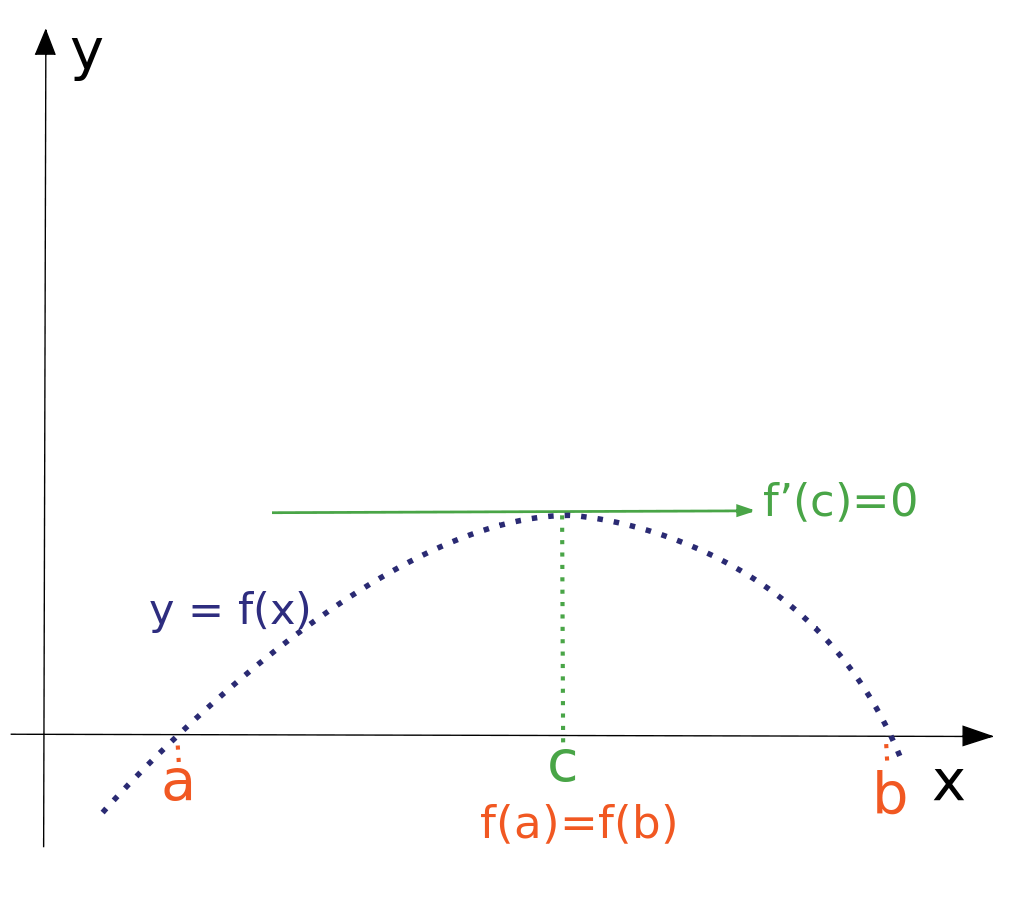
\includegraphics[scale=0.25, height=100px]{Figuras/rolle.png}
\end{figure}
\end{teorema}
\begin{teorema}[Valor Médio]

\end{teorema}
\end{tcolorbox}
\subsection*{Região de crescimento e concavidade. Esboço de gráficos}

\subsection*{ O Teorema de Taylor; a aproximação polinomial. }
\subsection*{Problemas de otimização}
\subsection*{Regra de L'Hospital}
\begin{tcolorbox}
Se $\lim\limits_{x\to a}\dfrac{f(x)}{g(x)}=\dfrac{0}{0} \text{ ou } \dfrac{\pm\infty}{\pm\infty}$ então
\begin{align*}
    \lim\limits_{x\to a}\dfrac{f(x)}{g(x)}=\lim\limits_{x\to a}\dfrac{f'(x)}{g'(x)}.
\end{align*}
\end{tcolorbox}
% % \subsection{Aplicações à química}
% % %\begin{center}
\textbf{Aplicações à Química}
\end{center}

As questões que seguem, foram retiradas do livro ``Matemática Ensino Médio Vol 1" de Luiz Roberto Dante.
\begin{enumerate}
\item A radioatividade é um fenômeno que ocorre em núcleos de átomos instáveis por emitirem partículas e radiações. A medida de tempo na qual metade da quantidade do material radioativo se desintegra é denominada meia-vida ou período de semidesintegração ($P$). A cada período de tempo $P$ a quantidade de material radioativo cai à metade da anterior, sendo possível relacionar a quantidade de material radioativo a qualquer tempo com a quantidade inicial por meio de uma função exponencial: 
$$N(t)=N_0 . \left(\dfrac{1}{2}\right)^{\frac{t}{p}},$$
em que $N_0$ é a quantidade inicial do material radioativo, $t$ é o tempo decorrido e $P$ é o valor da meia-vida do material radioativo considerado. A radioatividade faz parte de nossa vida, como quando se faz uma tomografia. Um dos isótopos mais usados nos radiofármacos injetados nos pacientes submetidos à tomografia é o carbono 11, cuja meia-vida é de 20 minutos. Qual o tempo necessário, em minutos, para que uma amostra de carbono 11 se reduza a $\dfrac{1}{4}$ do que era quando foi obtida?

\item O carbono 14 é um isótopo raro do carbono presente em todos os seres vivos. Com a morte, o nível de C14 no corpo começa a decair. Como é um isótopo radioativo de meia-vida de 5730 anos, e como é relativamente fácil saber o nível original de C14 no corpo dos seres vivos, a medição da atividade de C14 em um fóssil é uma técnica muito utilizada para datações arqueológicas. A atividade radioativa do C14 decai com o tempo pós-morte segundo a função exponencial
\[A(t)=A_0 . \left(\dfrac{1}{2}\right)^{\frac{t}{5730}},\]
em que $A_0$ é a atividade natural do C14 no organismo vivo e $t$ é o tempo decorrido em anos após a morte. Suponha que um fóssil encontrado em uma caverna foi levado ao laboratório para ter sua idade estimada. Verificou-se que emitia 7 radiações de C14 por grama/hora. Sabendo que o animal vivo emite 896 radiações por grama por hora, qual é a idade aproximada desse fóssil?

\item Os átomos de um elemento químico radioativo têm uma tendência natural a se desintegrar (emitindo partículas e se transformando em outros elementos). Dessa forma, com o passar do tempo, a quantidade original desse elemento diminui. Chamamos de meia-vida o tempo que o elemento radioativo leva para desintegrar metade de sua massa radioativa. O antibiótico acetilcefuroxina apresenta meia-vida de 3 horas. Se uma pessoa tomou 50mg desse medicamento, qual é a quantidade de antibiótico ainda presente no organismo:
\begin{enumerate}
\item após 12 horas de sua ingestão?
\item após t horas de sua ingestão?
\end{enumerate}

\item Considere uma substância radioativa de meia-vida $P$ que inicia o processo de desintegração. Que porcentagem de sua massa ainda restará após metade de sua primeira meia-vida?

\item Quando se administra um remédio, sua concentração no organismo deve oscilar entre dois níveis, pois não pode ser tão baixa a ponto de não fazer efeito (\emph{Ce}) e não pode ser tão alta a ponto de apresentar efeitos indesejáveis (toxicidade) ao paciente (\emph{Cp}). Quando, após um certo tempo depois de ministrado o remédio, o nível de concentração no organismo atinge \emph{Ce}, toma-se mais uma dose do remédio a fim de elevar o nível de concentração para \emph{Cp}. Esse tempo entre as administrações das doses é chamado de \emph{tempo interdoses}. É importante notar que o tempo interdoses, após a primeira medição, é o tempo que decorre para a concentração máxima tolerada \emph{Cp} decair até a concentração mínima eficaz \emph{Ce}.

Lembrando que a concentração de uma droga no organismo, após um tempo \emph{t}, é dada por
\[C(t)=C_0 . \left(\dfrac{1}{2}\right)^{\frac{t}{p}},\]
em que $C_0$ é a quantidade inicial ingerida do remédio, \emph{t} é o tempo decorrido e \emph{P} é o valor da meia-vida da substância no organismo, obtenha em função de \emph{Ce, Cp e P}: (Use que $\log 2=0,30$)
\begin{enumerate}
\item o valor do tempo interdoses;
\item a concentração de remédio $D$ nas doses que devem ser administradas ao paciente a cada intervalo interdoses.
\end{enumerate}
\end{enumerate}

% % \section{Software}
% % \input{Software/sage}
\section{Respostas}
\input{respostas}

%----------------------------------------------------------------------------------------

\end{document}